\documentclass[referee]{svjour3}


\usepackage{engsymbols}
\usepackage{magref}
\usepackage[utf8]{inputenc}
\usepackage[T1]{fontenc}
\usepackage{nicefrac}

\newcommand{\bmax}{\ensuremath{{B}\ped{max}}}
\newcommand{\bmin}{\ensuremath{{B}\ped{min}}}
\newcommand{\mrate}{\rate{m}}
\newcommand{\wvalven}{\w\ped{valve,n}}
\newcommand{\wrelayn}{\w\ped{relay,n}}

\usepackage{mathptmx}
\journalname{Journal of the Brazilian Society of Mechanical Sciences and Engineering}

\usepackage{graphicx}
\usepackage{subfig}
\usepackage{xcolor}
\usepackage{nomencl}
\usepackage{hyperref}

\begin{document}

\title{Numerical analysis of the influence of magnetic field waveforms on the performance of active magnetic regenerators}

\author{
Fábio P. Fortkamp \and
Gusttav B. Lang \and
Jaime A. Lozano \and
Jader R. Barbosa Jr.
}


\institute{
Fábio P. Fortkamp \\
\email{fabio@polo.ufsc.br} \\
Gusttav B. Lang \and
Jaime A. Lozano \and
Jader R. Barbosa Jr.
\at
POLO --- Research Laboratories for Emerging Technologies in Cooling and Thermophysics, Department of Mechanical Engineering, Federal University of Santa Catarina, Florianópolis, SC, 88040-900, Brazil}


\date{}

\titlerunning{Analysis of magnetic field waveforms}
\maketitle

\begin{abstract}
Magnetic cooling is an alternative to vapor compression with no use of hazarduous gases. The refrigerant is a solid material which reacts to oscillations in magnetic field with changes in temperature. In active magnetic regenerators, this magnetocaloric material and its effect are coupled with an oscillating fluid flow to yield a thermodynamic cooling cycle between cold and hot source temperatures. The literature is abundant with studies on the influence of the fluid flow waveform on magnetic refrigeration devices, but the influence of the magnetic field waveform is less investigated. In this work, we simulate a previously developed active magnetic regenerator numerical model with different mathematically-defined waveforms, and determine which operating parameters yield the highest values for cooling capacity and coefficient of performance. Results show that the highests performance levels are achieved when the magnetic field is kept constant for the same duration of the fluid flow through the magnetized material, and that the transition times between high and low levels of the magnetic field should be as fast as possible.

\keywords{ magnetic refrigeration \and active magnetic regenerator \and numerical modeling \and magnetocaloric effect}
\end{abstract}

\section{Introduction}
\label{sec:introduction}

Mechanical vapor compression has been the dominant cooling technology for the past century \cite{bib:nik} but, despite its dominance, it still faces an increasing number of challenges related to the its environmental footprint. In particular, the phase-out of refrigerants \textcolor{black}{with} ozone depleting \textcolor{black}{and global warming potentials has} introduced the use of flammable substances, with their own set of risks for consumer applications \cite{bib:iir-flammable} and technological challenges \cite{bib:lionte18-adapt}.

Magnetic refrigeration (MR) is an advanced cooling technology with no use of hazarduous gases, where a \emph{magnetocaloric material} (MCM) \textcolor{black}{is subjected to a cyclical change of the applied} magnetic field, and its temperature \textcolor{black}{changes as a result} of the \emph{magnetocaloric effect} (MCE). The magnitude of the MCE  \textcolor{black}{depends} on  material parameters, magnetic field variation and temperature, and its maximal at the Curie temperature of the material. For a thorough introduction to the magnetocaloric effect and magnetocaloric materials, the reader is referred to \cite{bib:smith-magneto}.


\nomenclature[vm]{MR}{Magnetic (or Magnetocaloric) Refrigeration}
\nomenclature[vm]{MCM}{Magnetocaloric Material}
\nomenclature[vm]{MCE}{Magnetocaloric Effect}

For operating conditions typical of a low-temperature span magnetic refrigerator, the MCE is typically \textcolor{black}{on} the order of \num{2}-\SI{5}{\kelvin}. \textcolor{black}{T}o amplify this \textcolor{black}{temperature change}, heat regeneration is usually employed \cite{bib:kitanovski}. Active magnetic regenerators (AMR) are thermal devices where the magnetocaloric material constitutes a solid matrix through which flows an aqueous heat transfer fluid, and which is cyclically magnetized and demagnetized to activate the magnetocaloric effect.  \textcolor{black}{Such a regenerator is essentially a cascade of infinitesimal ``layers'' of MCM that are activated simultaneously} to build up a temperature profile \textcolor{black}{along its length}. These layers can be made of the same material, yielding an homogeneous regenerator; however, given the  dependence  of the MCE with temperature, it is an interesting strategy to build \emph{multilayer} regenerators, where each layer is composed of a different material \textcolor{black}{that} will work around its \textcolor{black}{own} Curie temperature, maximizing the magnetocaloric effect of each portion.

\nomenclature[vm]{AMR}{Active Magnetic Regenerator}


Magnetic refrigerators can operate according to different thermodynamic cycles, but the stages are roughly as follows. The magnetic circuit magnetizes the MCM, increasing its temperature due to the MCE. During the so-called \emph{cold blow}, cold fluid from the cold source flows through the warm bed and absorbs its energy, releasing it to the external heat exchanger. On the return of the fluid, the solid is demagnetized and cooled down, and in the \emph{hot blow} the fluid relases energy to the bed, decreasing its temperature so it can absorb the thermal load at the cold source. The cycle then repeats; different cycles can be configured by different durations and synchronization steps between these two \emph{characteristic waveforms}:

\begin{enumerate}
\item The \emph{magnetic profile}, which describes the oscillating magnetic field over one regenerator;
\item The \emph{fluid flow profile}, which describes the time-variation of flow rate through one bed.
\end{enumerate}

Fluid flow profiles are more easily investigated with experimental methods, since they can be altered with modifications in the fluid flow system. In particular, the \emph{duration} of blows have been extensively investigated \cite{bib:teyber17_exper,bib:nakashima18-influen-exp,FORTKAMP2018}, and the literature shows that the cooling capacity of magnetic refrigerators can be increased by focusing fluid flows during periods where the magnetic field is at its extrema values.

In this work, we focus on magnetic profiles, which are less studied in the literature.
These waveforms are usually investigated in terms of their synchronization with the fluid flow profile \cite{TUSEK20111507,bib:bjoerk11_amr}. This paper uses the AMR model developed by \cite{bib:trevizoli16_perfor_model}, and the same authors had studied magnetic profiles waveforms in an earlier work \cite{bib:asme-mce}. However, their amplitudes was not varied, nor were they investigated with different geometries.

The present work combines the gaps from the above cited papers in investigating the performance of a magnetic refrigerator under different magnetic profile waveforms. These waveforms are mathematically modeled, and the cooling capacity and coefficient of performance are calculated based on the profiles parameters, while also investigated how the AMR geometry affect the performance in combinations with the magnetic profile. The fluid flow profile is assumed fixed in shape, although its parameters are also varied. To emulate constraints on an operating point of actual magnetic refrigeration devices, the temperature span is set fixed, and hence few comments are made on second-law efficiency.



\section{Materials and methods}
\label{sec:materials-methods}

In this work, we perform numerical simulations of a previously developed AMR model, varying the profile and geometric parameters. We also couple a model for calculating  the power comsumption of a proposed valve system, a topic understudied in the literature. With this, we can evaluate the influence of the profile on cooling capacity and coefficient of performance.

\subsection{AMR model}
\label{sec:amr-model}

\subsubsection{Governing equations}
\label{sec:governing-equations}

Simulations were performed using a one-dimensional AMR mathematical model \cite{bib:asme-mce,bib:trevizoli16_perfor_model}. Here we will show a summarized version focusing on the governing equations. This model solves momentum and energy balance equations for the solid and fluid phases, represented by indices 's' and 'f', respectively. The model geometry is depicted in \autoref{fig:amrmodel}, and assumes regenerators composed of monodisperse packed spheres with porosity $\varepsilon$.

\nomenclature[is]{s}{solid phase}
\nomenclature[if]{f}{fluid phase}

\begin{figure}[!ht]
  \centering
  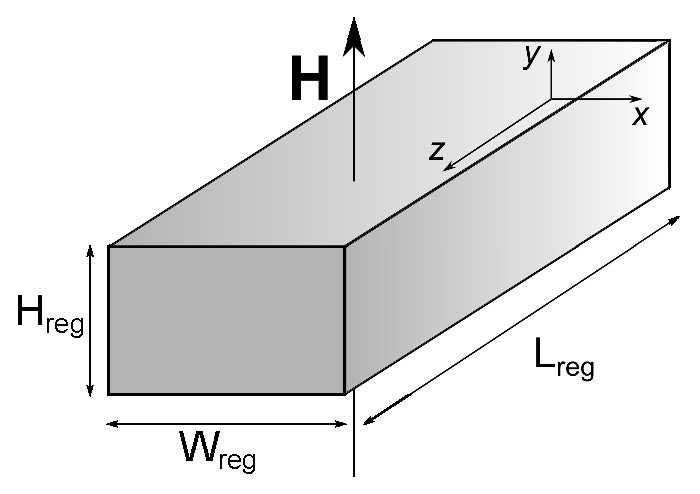
\includegraphics[width=8cm]{reg3d}
  \caption{AMR model geometry}
  \label{fig:amrmodel}
\end{figure}

The momentum equation for the fluid domain is:

\begin{equation}
\label{eq:75}
  \frac{\rho\ped{f}}{\varepsilon} \diffp{V_z}{t}= -\diffp{P}{z} - \frac{\mu\ped{f}}{K} V_z - \frac{c\ped{E} \rho\ped{f}}{K^{1/2}} \left| V_z\right| V_z 
\end{equation}

\nomenclature[ak]{$K$}{permeability of the porous medium [\si{\meter\square}]}
\nomenclature[ac]{$c\ped{E}$}{Ergun constant of the porous medium}
\nomenclature[ar]{$\rho$}{density [\si{\kg\per\cubic\meter}]}
\nomenclature[be]{$\varepsilon$}{porosity}
\nomenclature[av]{$V$}{velocity [\si{\meter\per\second}]}
\nomenclature[ap]{$P$}{pressure [\si{\pascal}]}
\nomenclature[bu]{$\mu$}{dynamic viscosity [\si{\pascal\second}]}


\noindent and is solved for the time-dependent uniform fluid velocity through the bed. 

The energy equation for the fluid phase can be written as:

\begin{equation}
\label{eq:78}
\begin{split}
  \rho\ped{f} c_{p,\mathrm{f}} \left(\varepsilon \diffp{T\ped{f}}{t} + V_z\diffp{T\ped{f}}{z}\right) = & -\hheat\ped{sf} \beta \left(T\ped{f} - T\ped{s}\right) \\
& + \left|V_z\diffp{p}{z}\bigg|_f \right| \\
& + \varepsilon\left(k\ped{f}\ap{eff}  +\rho\ped{f} c_{p,\mathrm{f}} D\ped{ld}\right)\diffp[2]{T\ped{f}}{z} \\
& + \rate{q}\ped{csg}  
\end{split}
\end{equation}

\nomenclature[at]{$T$}{temperature [\si{\kelvin}]}
\nomenclature[at]{$t$}{time [\si{\second}]}
\nomenclature[az]{$z$}{axial coordinate [\si{\meter}]}

\nomenclature[aq]{$\rate{q}\ped{csg}$}{volumetric casing losses in the AMR model [\si{\watt\per\cubic\meter}]}
\nomenclature[ic]{csg}{regenerator casing}
\nomenclature[ah]{$\hheat$}{heat transfer coefficient [\si{\watt\per\meter\squared\per\kelvin}]}
\nomenclature[aa]{$A\ped{sf}$}{contact surface area between solid and fluid phases in the regenerator [\si{\meter^2}]}
\nomenclature[is]{sf}{relative to the heat transfer between solid and fluid phases in the regenerator}
\nomenclature[azb]{$\beta$}{surface area density [\si{\squared\meter\per\cubic\meter}]}
\nomenclature[ak]{$k\ap{eff}$}{effective thermal conductivity [\si{\watt\per\meter\per\kelvin}]}
\nomenclature[ad]{$D\ped{ld}$}{dispersion term in the AMR model [\si{\meter\square\per\second}]}
\nomenclature[af]{$f$}{cycle frequency [\si{\hertz}]}
\nomenclature[azf]{$\Phi$}{utilization}
\nomenclature[am]{$m$}{mass [\si{\kg}]}

\nomenclature[azt]{$\tau$}{time period [\si{\second}]}
\nomenclature[ac]{$c$}{specific heat [\si{\joule\per\kg\per\kelvin}]}


\noindent while the energy equation for the solid phase is written as:

\begin{equation}
\label{eq:88}
  \rho\ped{s} c\ped{s}(1 - \varepsilon)\diffp{T\ped{s}}{t} = \hheat\ped{sf}\beta(T\ped{f}-T\ped{s}) + (1-\varepsilon)k\ped{s}\ap{eff}\diffp[2]{T\ped{s}}{z}
\end{equation}

Initial and boundary conditions, solution methods, convergence analyses, and closure relations for the porous media terms are described in \cite{bib:trevizoli16_perfor_model}. This AMR model solves the above equations for one regenerator operating between given sources temperatures, during one full cycle (hot and cold blows and  magnetization and demagnetization periods), given specified operating conditions (to be discussed later).

The casing heat transfer term $\rate{q}\ped{csg}$ in \autoref{eq:78} is calculated solving the heat conduction in the regenerators casing \cite{bib:trevizoli16_perfor_model}, and can be neglected to simplify some analyses. More details are provided in \autoref{sec:results-discussions}.

\subsubsection{How the fluid flow profile is used}
\label{sec:how-fluid-flow}

The pressure gradient in \autoref{eq:75}is modeled as:

\begin{equation}
\label{eq:76}
-\diffp{P}{z} = \rho\ped{f} A\ped{t} g(t)
\end{equation}

\noindent where \(g(t)\) is a dimensionless function that expresses the mathematical waveform of the pressure gradient, and  \(A\ped{t}\) is its amplitude,  adjusted in a convergence loop; the mass flow rate calculated from the Darcy velocity from \autoref{eq:75} is compared with the input value of mass flow rate until these values converge. The waveform $g(t)$ represents the fluid flow profile used.

\nomenclature[ag]{$g(t)$}{dimensional waveform of the pressure gradient term in the fluid momentum equation}
\nomenclature[aA]{$A\ped{t}$}{amplitude of the pressure gradient waveform in the fluid momentum equation [\si{\meter\per\second\square}]}


\subsubsection{How the magnetic profile is used}
\label{sec:how-magnetic-profile}


The magnetic profile is modeled by a waveform of magnetic field strength $H$ applied perpendicular to the regenerators, as shown in \autoref{fig:amrmodel}. The magnetic field is assumed uniform throughout the beds. The applied field is corrected from demagnetization effects to yield the effective field inside the regenerators:

\begin{equation}
  \label{eq:6}
  H\ap{eff} = H - N\ped{D} M
\end{equation}

\nomenclature[am]{$M$}{magnetization field [\si{\ampere\per\meter}]}
\nomenclature[an]{$N\ped{D}$}{demagnetization tensor}

\noindent where $M$ is the magnetization field of the material, and $N\ped{D}$ is a demagnetization factor.

The magnetocaloric effect is implemented in the so-called discrete approach \cite{bib:nielsen11_review}; every time the magnetic field changes, based on the input magnetic profile, the solid temperature is calculated according to:

\begin{equation}
  \label{eq:89}
  T\ped{s}(t + \Delta{}t) = T\ped{s}(t) + \dtad \left(T\ped{s}(t),H\ap{eff}(t),H\ap{eff}\left(t + \Delta{}t\right)\right)
\end{equation}


\nomenclature[ct]{$\dtad$}{adiabatic temperature variation [\si{\kelvin}]}

\noindent where the adiabatic temperature variation $\dtad$ is calculated from \textcolor{black}{tabulated} experimental \textcolor{black}{data} for magnetocaloric materials as function of temperature and effective field. \cite{bib:trevizoli16_perfor_model}.

\subsubsection{Evaluation of solid and fluid properties}
\label{sec:eval-solid-fluid}

The fluid properties are considered constant in the momentum equation to decouple the solution \textcolor{black}{procedures to determine} the velocity and temperature fields. The properties are computed at the average temperature between the hot and cold sources temperatures, and are evaluated from interpolated tables exported from the EES software \cite{bib:klein13-ees}. In all simulations shown in this work, the heat transfer fluid is a mixture of water/ethylene-glycol with concentration \num{80}/\SI{20}{\percent} vol. For the energy equations, the fluid properties are also calculated from tabulated data, but the temperature dependence is considered.

n this chapter, all simulations use gadolinium or its allows as the magnetocaloric material. Gadolinium is a benchmark material with a Curie temperature of \SI{290}{\kelvin}. \textcolor{black}{For simplicity, the solid} density is assumed constant at $\rho\ped{s} = \SI{7900}{\kg\per\cubic\meter}$ and the solid \textcolor{black}{thermal} conductivity is set to $k\ped{s} = \SI{10.5}{\watt\per\meter\per\kelvin}$. The specific heat \textcolor{black}{capacity} of \ce{Gd} is calculated as a function of temperature and magnetic field based on experimental \textcolor{black}{data}, using a bi-linear interpolation scheme; more details on the experimental dataset \textcolor{black}{are available} in \cite{bib:trevizoli16_perfor_model}. 

In this work, both single- and multilayer regenerators are considered. For the multilayer simulations, alloys of gadolinium and yttrium are used in the form \ce{Gd_{1-x}Y_x}, where $x$ is the yttrium fraction.  \textcolor{black}{This fraction} decreases the Curie temperature  \textcolor{black}{of the} alloy relative to that of pure gadolinium. Due to the lack of experimental  \textcolor{black}{data on the magnetocaloric properties of} \ce{Gd_{1-x}Y_x} alloys at the time \textcolor{black}{this analysis was made}, a simpler approach was used \textcolor{black}{in which} the properties of alloys with {a} low yttrium fraction are \textcolor{black}{identical to those} of pure gadolinium, except for the Curie temperature \textcolor{black}{(which is shifted to lower values)}. 


\subsubsection{Performance metrics}
\label{sec:performance-metrics}

The AMR model considers only one bed and assumes $N\ped{r}$ identical beds experience the same cycle, multiplyind the performance metrics below by this factor

\nomenclature{an}{$N\ped{r}$}{number of regenerators}

The cooling capacity is calculated as \cite{bib:trevizoli16_perfor_model}:

\begin{equation}
\label{eq:99}
\qc = N\ped{r}\frac{1}{\tau} \int_{\tau\ped{HB}} \mrate\ped{f}(t) c_{p,\mathrm{f}} \left( T\ped{C} -T\ped{f,CE} \right) \diffd{t}
\end{equation}

\noindent where $\tau$ is the cycle period, and $\tau\ped{HB}$ is the duration of the hot blow, during which the cold end temperature is compared to the cold source temperature.

\nomenclature[vh]{HB}{hot blow}
\nomenclature[vc]{CE}{cold end}
\nomenclature[am]{$\mrate\ped{f}$}{mass flow rate [\si{\kg\per\second}]}
\nomenclature[vc]{C}{cold source}
\nomenclature[vc]{H}{hot source}

The magnetic power to operate the AMR cycle is modeled as the ideal Carnot power, ignoring most thermal irreversibilities:

\begin{equation}
\label{eq:100}
\wmag = \qc \frac{T\ped{H} - \tc}{\tc}
\end{equation}

\noindent while the fluid friction irreversibility is accounted for in the calculation of the pumping power:

\begin{equation}
\label{eq:103}
\wpump = N\ped{r}\frac{1}{\tau}\int_0^{\tau}\frac{\rate{m}\ped{f}}{\rho\ped{f}} \Delta P \diffd{t}
\end{equation}

\noindent where $\Delta P$ is the total pressure drop through the regenerator.

\nomenclature[awm]{$\wpump$}{pumping power [\si{\watt}]}
\nomenclature[awm]{$\wmag$}{magnetic power [\si{\watt}]}
\nomenclature[ap]{$\Delta P$}{pressure drop across one region [\si{\pascal}]}

\subsection{Hydraulic system  and fluid flow profile model}
\label{sec:hydr-syst-model}

The canonical fluid flow profile considered in this work \textcolor{black}{ is the square wave or \emph{instantaneous profile}}, because of the instantaneous change in flow rate, as shown in \autoref{fig:mprofile}. 

\begin{figure}[!ht]
  \centering
  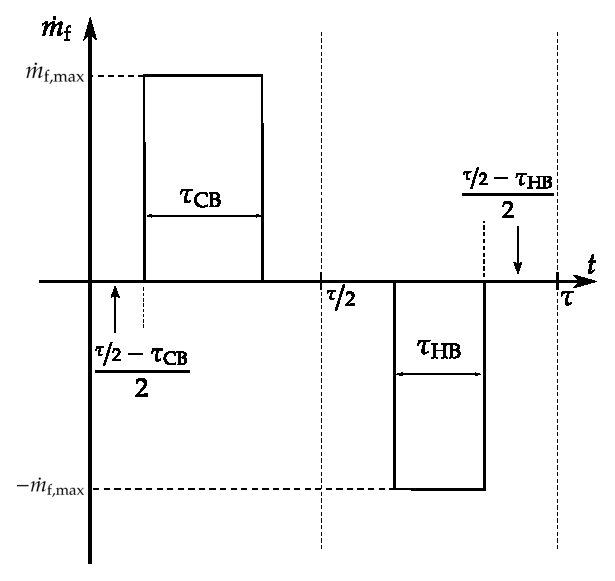
\includegraphics[width=8cm]{mprofile}
  \caption{Instantaneous fluid flow profile}
  \label{fig:mprofile}
\end{figure}

The \textcolor{black}{instantaneous mass flow rate}, \(\rate{m}\ped{f}(t)\), is defined over a cycle with \textcolor{black}{a} period \(\tau\), and represents the fluid flow \textcolor{black}{through} a given regenerator bed. The so-called \emph{hot cycle}, \textcolor{black}{during which} the MCM is magnetized, occupies the \textcolor{black}{time interval} \(0 \le t < \nicefrac{\tau}{2}\), while the \emph{cold cycle}
lies \textcolor{black}{between} \(\nicefrac{\tau}{2} \le t \le \tau\). The flow profile oscillates between two plateaus of equal magnitude
\(\rate{m}\ped{f,max}\) \textcolor{black}{and} opposite directions, \textcolor{black}{which} are centered in each half-cycle. During the hot cycle, the cold
blow period is \(\tau\ped{CB}\), and during the cold cycle the hot blow period is \(\tau\ped{HB}\). If the flow is balanced, then \(\tau\ped{CB} = \tau\ped{HB}\).


During each half cycle, there are periods \textcolor{black}{without}  fluid flow, defined as:

\begin{equation}
\label{eq:48}
\tau\ped{0,HC} = \frac{\nicefrac{\tau}{2} - \tau\ped{CB}}{2}
\end{equation}

\begin{equation}
\label{eq:49}
\tau\ped{0,CC} = \frac{\nicefrac{\tau}{2} - \tau\ped{HB}}{2}
\end{equation}

where HC and CC stand for hot \textcolor{black}{cycle} and cold cycle, respectively.

\nomenclature[vh]{HC}{hot cycle}
\nomenclature[vc]{CC}{cold cycle}

The profile can be mathematically defined as:

\begin{equation}
\rate{m}\ped{f}(t)=
\begin{cases}
0, & 0 \le t < \tau\ped{0,HC} \\
\rate{m}\ped{f,max}, & \tau\ped{0,HC} \le t \le \nicefrac{\tau}{2} - \tau\ped{0,HC} \\
0, & \nicefrac{\tau}{2} - \tau\ped{0,HC} < t < \nicefrac{\tau}{2} + \tau\ped{0,CC} \\
-\rate{m}\ped{f,max}, & \nicefrac{\tau}{2} + \tau\ped{0,CC} \le t \le \tau - \tau\ped{0,CC} \\
0, &  \tau - \tau\ped{0,CC} <  t < \tau \\
\end{cases}
\label{eq:50}
\end{equation}

When the blows have different time durations, the AMR cycle is considered unbalanced, and this \textcolor{black}{is known to have} a negative effect on performance \cite{bib:eriksen16_effec,bib:nakashima18-influen-exp}. In this work, the blows are always balanced, hence the blow fraction, the ratio of blow durations to cycle period \cite{bib:nakashima18-influen-exp}, can be evaluated as:

\begin{equation}
\label{eq:59}
F\ped{B} = \frac{2\tau\ped{B}}{\tau}
\end{equation}

\noindent where $\tau\ped{B}$ is the duration of one blow.

\nomenclature[azt]{$\tau\ped{B}$}{blow duration [\si{\second}]}

The hydraulic system to modulate this fluid flow through different regenerators at different time instants is composed of a pump and a set of electronic valves which can be precisely controlled to yield the desired blow durations. The electrical power consumed by the valve array is computed separately from other work contributions. An application of electronic valves in AMR devices has been presented by \cite{bib:nakashima18-perfor-asses-solen-valves-flow}.

Due to evolving developments in our group, two types of valves are considered, as will be elaborated in \autoref{sec:results-discussions}.

The first approach, called \emph{Type B valves}, uses the  model \textcolor{black}{of} \cite{bib:cardoso16_trans}, assuming that the individual consumption of each valve is independent of frequency and blow fraction. The valve power  $\wvalve$ can be computed as:

\begin{equation}
  \label{eq:58}
  \wvalve = N\ped{v}F\ped{B}\left(\wvalven + \frac{1}{2}\wrelayn\right)
\end{equation}

\noindent where $N\ped{v}$ is the number of valves, $\wvalven$ is the measured average nominal power for one normally-closed electronic valve and $\wrelayn$ is the nominal power for one controlling relay. The factor $\nicefrac{1}{2}$ is due to two valves being controlled by one relay.

\nomenclature[an]{$N\ped{v}$}{number of valves}
\nomenclature[aw]{$\wvalve$}{valve power [\si{\watt}]}
\nomenclature[aw]{$\wvalven$}{nominal power comsumption of one valve [\si{\watt}]}
\nomenclature[aw]{$\wrelayn$}{nominal power comsumption of one relay [\si{\watt}]}

In the second approach, \emph{Type A} valves are used, with lower nominal power but that depends on frequency and blow fraction. For these valves, the valve power was experimentally correlated as:

\begin{equation}
  \label{eq:198}
  \wvalve\,[\si{\watt}]= N\ped{v}\left(0.927 f\,[\si{\hertz}] + 1.023 F\ped{B} + 0.226 f\,[\si{\hertz}] F\ped{B} - 0.037\right)
\end{equation}

Equation~\eqref{eq:198} was correlated for blow fractions of \num{50} and \SI{100}{\percent} and for frequencies in the range \textcolor{black}{of} \num{0.2}--\SI{1.6}{\hertz}, with an uncertainty \textcolor{black}{on} the order of \SI{0.4}{\watt} for a single valve. The use of different valve types will be discussed among the presented results.

Indepedent of the valve type used, it is also assumed that this valve system can produce the fluid flow profile \textcolor{black}{shown in} \autoref{fig:mprofile}, where the displaced fluid mass during one blow in one regenerator bed is $\rate{m}\ped{f,max} F\ped{B} \nicefrac{\tau}{2}$. 

The \emph{utilization factor} can then be calculated as:

\begin{equation}
  \label{eq:110}
  \Phi = \frac{\rate{m}\ped{f,max} F\ped{B} c\ped{s}}{2 f m\ped{s} c\ped{s}}
\end{equation}

\nomenclature[bf]{$\Phi$}{utilization factor}

\textcolor{black}{For an even number of poles in the magnetic circuit}, it may be advantageous to employ an odd number of regenerator beds to  \textcolor{black}{break the symmetry between the magnetic circuit and the beds, thus avoiding positions of equilibrium between magnetic forces which result in torque oscillations} \cite{bib:eriksen}. \textcolor{black}{Additionally}, in general, two valves per regenerator  may be necessary (one at each end), to independently control  the hot and cold blows for each bed and correct flow \textcolor{black}{imbalance}; thus, in all results in this work, the number of valves is \textcolor{black}{calculated as}:

\begin{equation}
  \label{eq:111}
  N\ped{v} = 2 N\ped{r}
\end{equation}

\subsection{Calculation of the coefficient of performance}
\label{sec:calc-coeff-perf}

The coefficient of performance \textcolor{black}{takes} the cooling capacity as \textcolor{black}{the main} output \textcolor{black}{parameter from} the AMR model, \textcolor{black}{in addition to} all previously cited power contributions:

\begin{equation}
  \label{eq:112}
  \cop = \frac{\qc}{\wpump + \wmag + \wvalve}
\end{equation}

\subsection{Definition of magnetic profiles}
\label{sec:defin-magn-prof}

The magnetic profiles considered in this work were shown in \autoref{fig:profiles}; here their mathematical definitions are presented. The profiles are presented in terms of the flux density $B = \mu_0 H$, where $\mu_0$ is the permeability of free space; the magnetic field $H$ is used in the evaluation of the magnetocaloric effect (cf. \autoref{sec:how-magnetic-profile}).

The instantaneous profile (represented by the subscript ``IT'') and the rectified cosine profile (represented by ``RC'') are defined solely in terms of the \textcolor{black}{(extreme)} values $B\ped{min}$ and $B\ped{min}$:

\nomenclature[vi]{IT}{instantaneous magnetic profile}
\nomenclature[vr]{RC}{rectified cosine magnetic profile}

\begin{equation}
{B}\ped{IT}\,(t)=
\begin{cases}
{B}\ped{max}, & 0 \le t < \nicefrac{\tau}{2} \\
{B}\ped{min}, & \nicefrac{\tau}{2} \le t < \tau\\
\end{cases}
\label{eq:199}
\end{equation}

\begin{equation}
{B}\ped{RC}\,(t) = B\ped{min} + \left(B\ped{max} - B\ped{min}\right)  \left\lvert \cos\left( \frac{\pi}{\tau} \left( t - \frac{\tau}{4}\right)\right) \right\rvert
\label{eq:200}
\end{equation}

As previously discussed, a suitable approximation of the instantaneous profile is the \textcolor{black}{\emph{magnetic ramp profile}, shown} in \autoref{fig:ramp}. The so-called \emph{hot cycle}, \textcolor{black}{during which} the MCM is magnetized, occupies the range \(0 \le t < \nicefrac{\tau}{2}\), while the \emph{cold cycle} lies in the range \(\nicefrac{\tau}{2} \le t < \tau\). The magnetic profile oscillates  between a low value \({B}\ped{min}\) and a high value \({B}\ped{max}\), and \textcolor{black}{remains} at each plateau for a period of \(\tau\ped{M}\). The plateaus are balanced and centered at each half-cycle.

\begin{figure}[!ht]
  \centering
  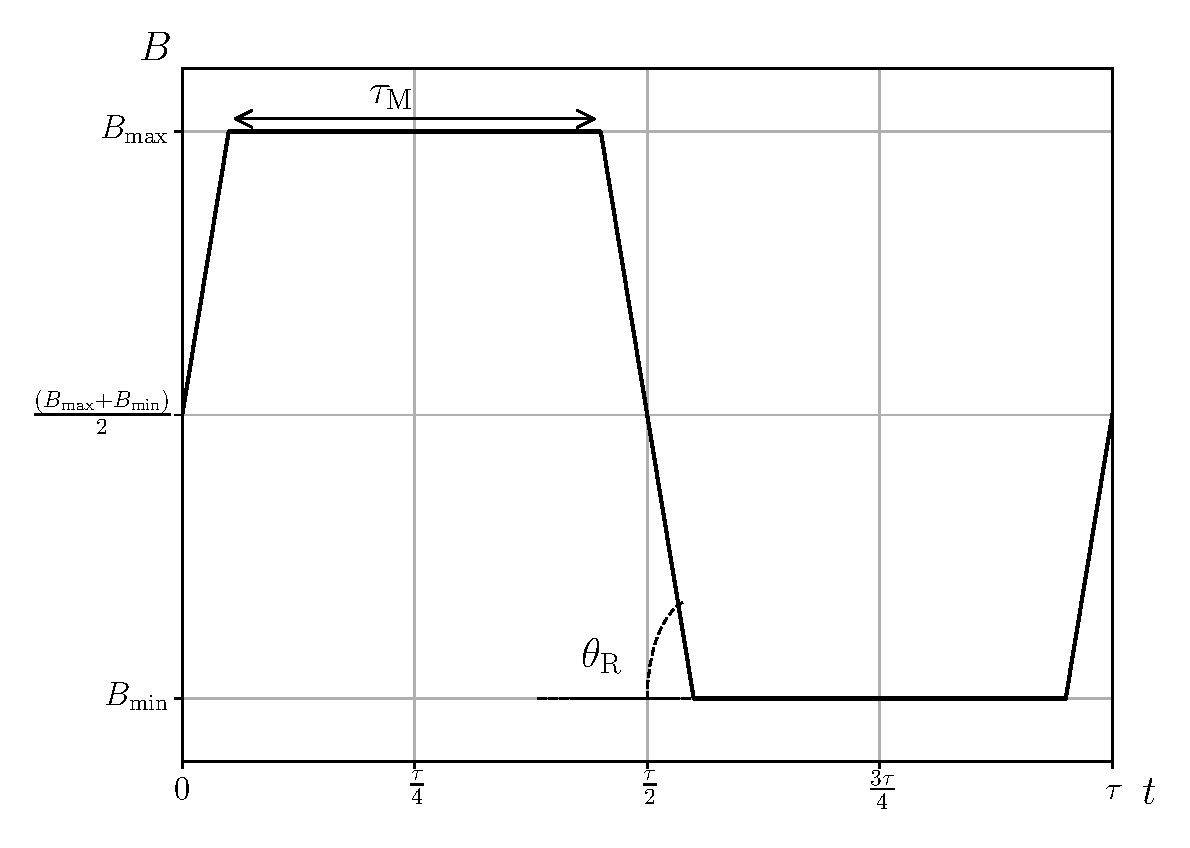
\includegraphics[width=7cm]{profile_rm}
  \caption{\textcolor{black}{Magnetic ramp}  profile}
  \label{fig:ramp}
\end{figure}

The \emph{ramp period} \(\tau\ped{R}\) \textcolor{black}{is} defined as:

\begin{equation}
\label{eq:201}
\tau\ped{R} = \frac{1}{4}\left(\tau - 2 \tau\ped{M}\right)
\end{equation}

\noindent such that there are four ramp periods in one full cycle. The ramp rate, \(\theta\ped{R}\), is:

\begin{equation}
\label{eq:202}
\tan \theta\ped{R} = \frac{\left({B}\ped{max} - {B}\ped{min}\right)}{2\tau\ped{R}}
\end{equation}

\nomenclature[azt]{$\tau\ped{R}$}{ramp period in the \textcolor{black}{magnetic} ramp profile [\si{\second}]}
\nomenclature[azt]{$\tau\ped{M}$}{magnetization period in the \textcolor{black}{magnetic} ramp  profile [\si{\second}]}
\nomenclature[azo]{$\theta\ped{R}$}{ramp rate in the \textcolor{black}{magnetic} ramp profile}

The magnetization fraction, \(F\ped{M}\), is the fraction of the cycle \textcolor{black}{during which} the magnetocaloric material is \textcolor{black}{subjected to a} constant magnetic field:

\begin{equation}
\label{eq:204}
F\ped{M} = \frac{2\tau\ped{M}}{\tau}
\end{equation}

\nomenclature[af]{$F\ped{M}$}{magnetization fraction}

The ramp profile (``RM'') can be mathematically defined as:

\begin{equation}
{B}\ped{RM}(t)=
\begin{cases}
\nicefrac{\left({B}\ped{max} + {B}\ped{min}\right)}{2} + t \tan \theta\ped{R} , & 0 \le t < \tau\ped{R} \\
{B}\ped{max}, & \tau\ped{R} \le t < \nicefrac{\tau}{2} - \tau\ped{R}\\
{B}\ped{max} - \left(t - \left(\nicefrac{\tau}{2} - \tau\ped{R}\right)\right) \tan \theta\ped{R} , & \nicefrac{\tau}{2} - \tau\ped{R} \le t < \nicefrac{\tau}{2} + \tau\ped{R} \\
{B}\ped{min}, & \nicefrac{\tau}{2} + \tau\ped{R} \le t < \tau - \tau\ped{R}\\
{B}\ped{min} + \left(t - \left(\tau - \tau\ped{R}\right)\right) \tan \theta\ped{R} , & \tau - \tau\ped{R} \le t \le \tau \\
\end{cases}
\label{eq:203}
\end{equation}

\nomenclature[vr]{RM}{rectified cosine magnetic profile}

Additionally, the average values of the magnetic field during each half-AMR cycle are considered for comparison between profiles. The average magnetic profile during the hot cycle ($0 \le t < \nicefrac{\tau}{2}$) is denoted $\average{B}\ped{high}$ and the average during the cold cycle  ($ \nicefrac{\tau}{2} \le t < \tau$) is denoted $\average{B}\ped{low}$. For the instantaneous waveform, these average values are identical to the extrema values.


\section{Results and Discussions}
\label{sec:results-discussions}

The analysis of magnetic profiles was performed in two different stages in the research of our group, as discussed below.

\subsection{Comparison of instantaneous and rectified cosine profiles using a simplified model}
\label{sec:comp-cosine-inst}

In the first stage, the instantaneous and rectified cosine profiles are compared in the AMR model, considering monolayer regenerators without casing losses, and using Type B valves. The parameters used in all simulations are presented in \autoref{tab:params-cobem}.

\begin{table}[!ht]
  \centering
  \caption{AMR parameters kept fixed in the simulations with different magnetic profiles}
  \begin{tabular}{c|c}
\hline
\textbf{Parameter} & \textbf{Value}\\
\hline
   $D\ped{p}$ & \SI{0.5}{\mm}\\
$H\ped{r}$ & \SI{20}{\mm}\\
$W\ped{r}$ & \SI{25}{\mm}\\
$L\ped{r}$ & \SI{100}{\mm}\\
$N\ped{r}$ & 11 \\
$N\ped{v}$ & 22 \\
$T\ped{H}$ & \SI{298}{\kelvin}\\
$\tc$ & \SI{278}{\kelvin}\\
$\w\ped{NV}$ & \SI{4}{\watt}\\
$\w\ped{R}$ & \SI{0.36}{\watt}\\
\hline
  \end{tabular}

  \label{tab:params-cobem}
\end{table}


When comparing the \textcolor{black}{performances resulting from the application of the different} magnetic profiles, the average magnetic field during the hot cycle \textcolor{black}{will be considered} the same; this implies a higher peak for the rectified cosine. For the cold cycle, two comparison methods are considered, as shown in \autoref{fig:comparison-methods-profiles}:

\begin{enumerate}
\item The minimum values for both profiles is the same;
\item The average value for both profiles during the cold cycle is the same.
\end{enumerate}


\textcolor{black}{For} reference, in all simulations,  the minimum value for the rectified cosine was fixed at ${B}\ped{min,RC} = \SI{0.1}{\tesla}$. \textcolor{black}{In} the first comparison, the minimum value for the instantaneous \textcolor{black}{waveform} was kept at the same level (${B}\ped{min,IT} =  {B}\ped{min,RC}$); hence, the average low value for the RC profile was higher ($\average{B}\ped{low,RC} > \average{B}\ped{low,IT}$). This represents common design scenarios: a constant low-valued plateau for the magnetic field for instantaneous-like magnetic profiles \cite{bib:insinga16_optim,bib:benedict16_desig}, or a low peak for the rectified cosine profile \cite{bib:trevizoli15_desig_halbac}.  For the other comparison method, the low level of the instantaneous profile was increased (${B}\ped{min,IT} >  {B}\ped{min,RC}$) \textcolor{black}{in order} to keep the \textcolor{black}{same} average ($\average{B}\ped{low,RC} = \average{B}\ped{low,IT}$). 




\begin{figure}[!ht]
  \centering
  \subfloat[Same minimum]{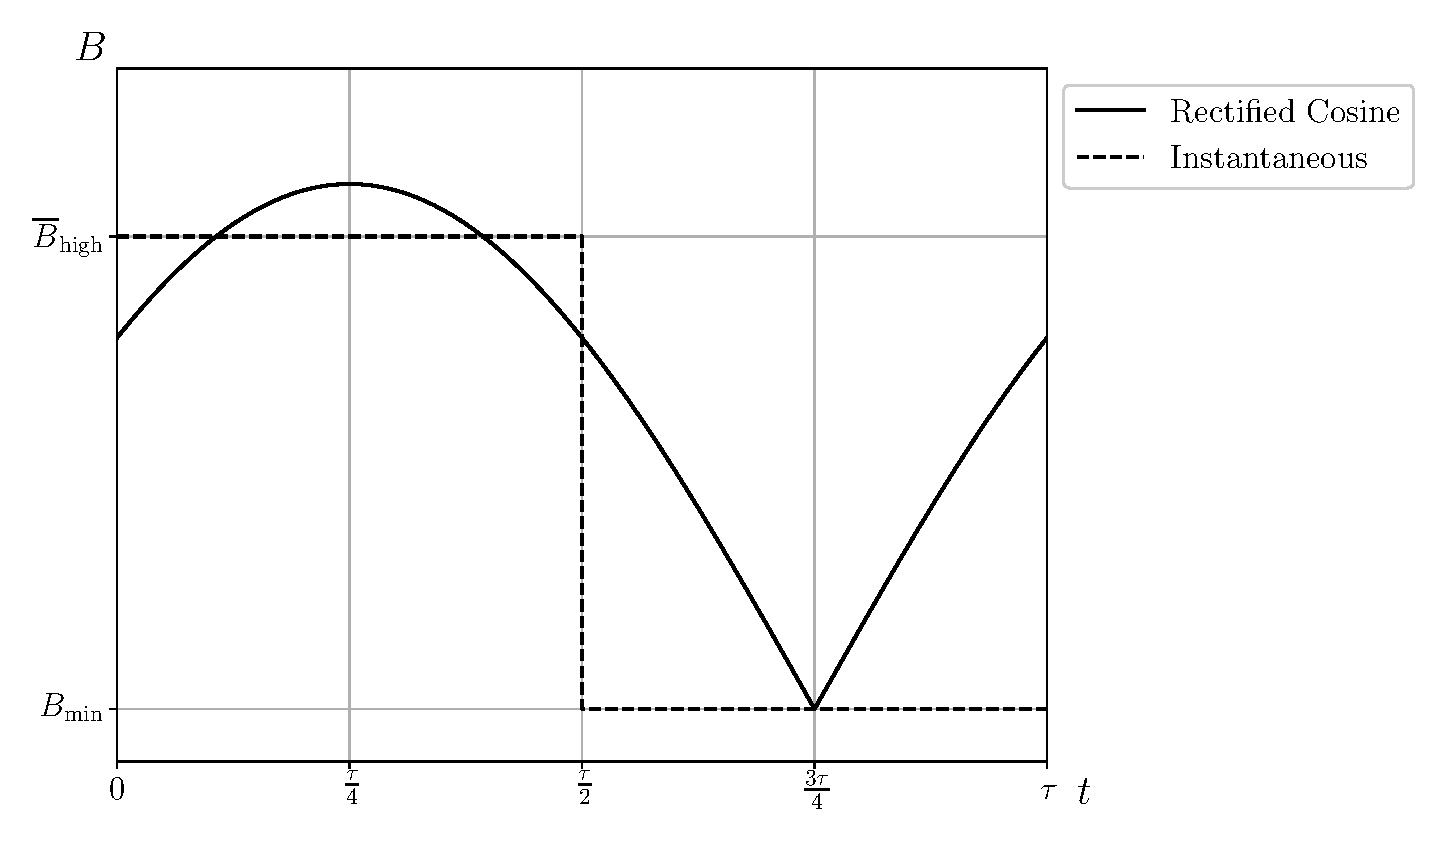
\includegraphics[width=8cm]{profiles_it_and_rc_same_minimum}\label{fig:profiles_inst_cos_same_minimum}}
\quad
  \subfloat[Same average]{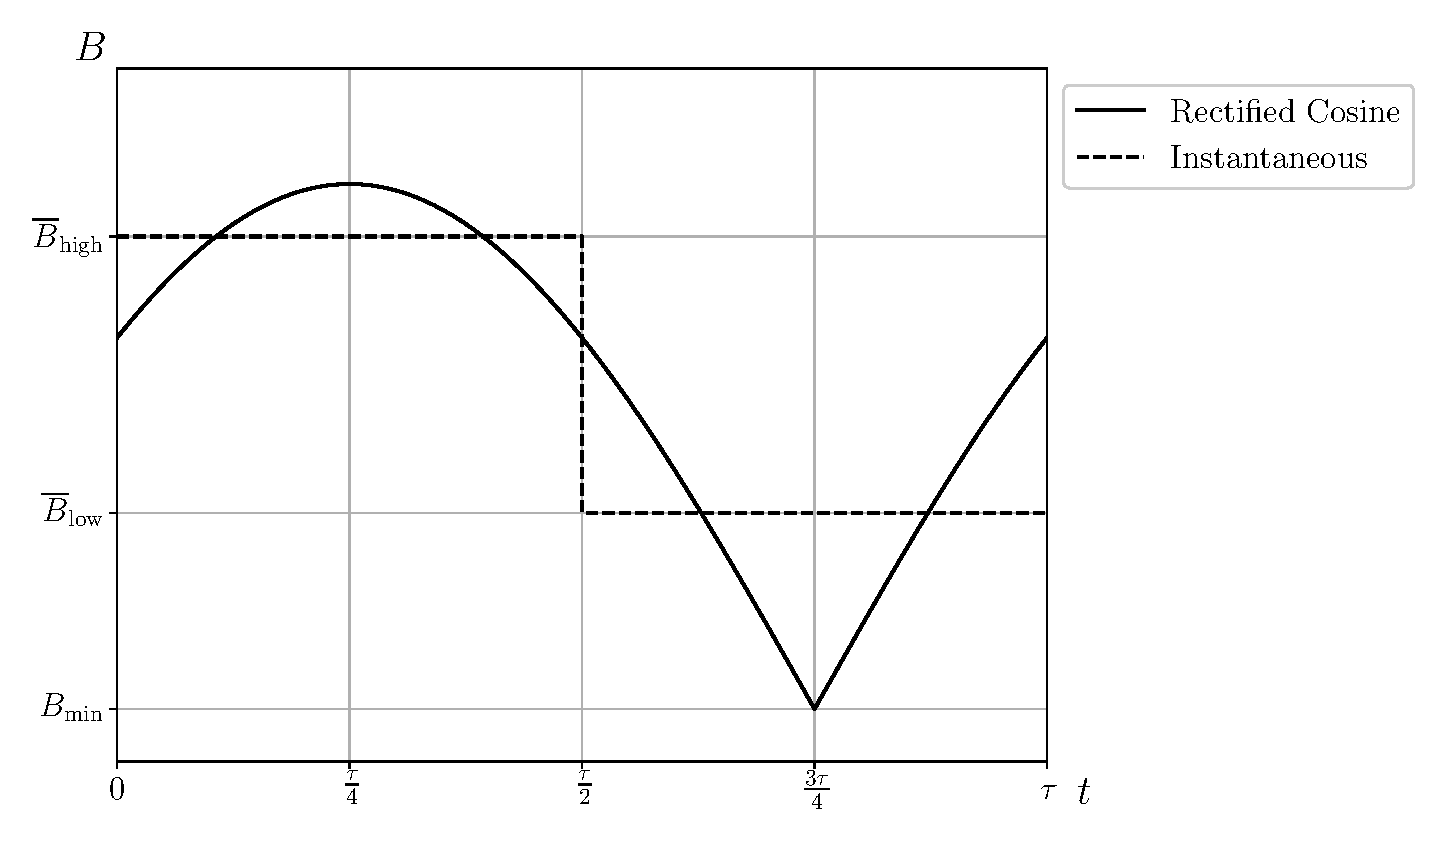
\includegraphics[width=8cm]{profiles_it_and_rc_same_average}\label{fig:profiles_inst_cos_same_average}}
  \caption{Comparison methods for the instantaneous and rectified cosine profiles }
  \label{fig:comparison-methods-profiles}
\end{figure}

In addition, simulations were \textcolor{black}{carried out} for various values of blow fraction; the rectified cosine profile can benefit from a smaller blow fraction because this can concentrate the flow during the periods of very high or low fields. In this section, all results use the critical value of blow fraction that maximized the cooling capacity: fluid flowing during the entire period for the instantaneous profile, and only during \SI{60}{\percent}  of the period (the smallest blow fraction tested) for the cosine profile; this latter case is shown in \autoref{fig:cos-inst-60}.

\begin{figure}[!ht]
  \centering
  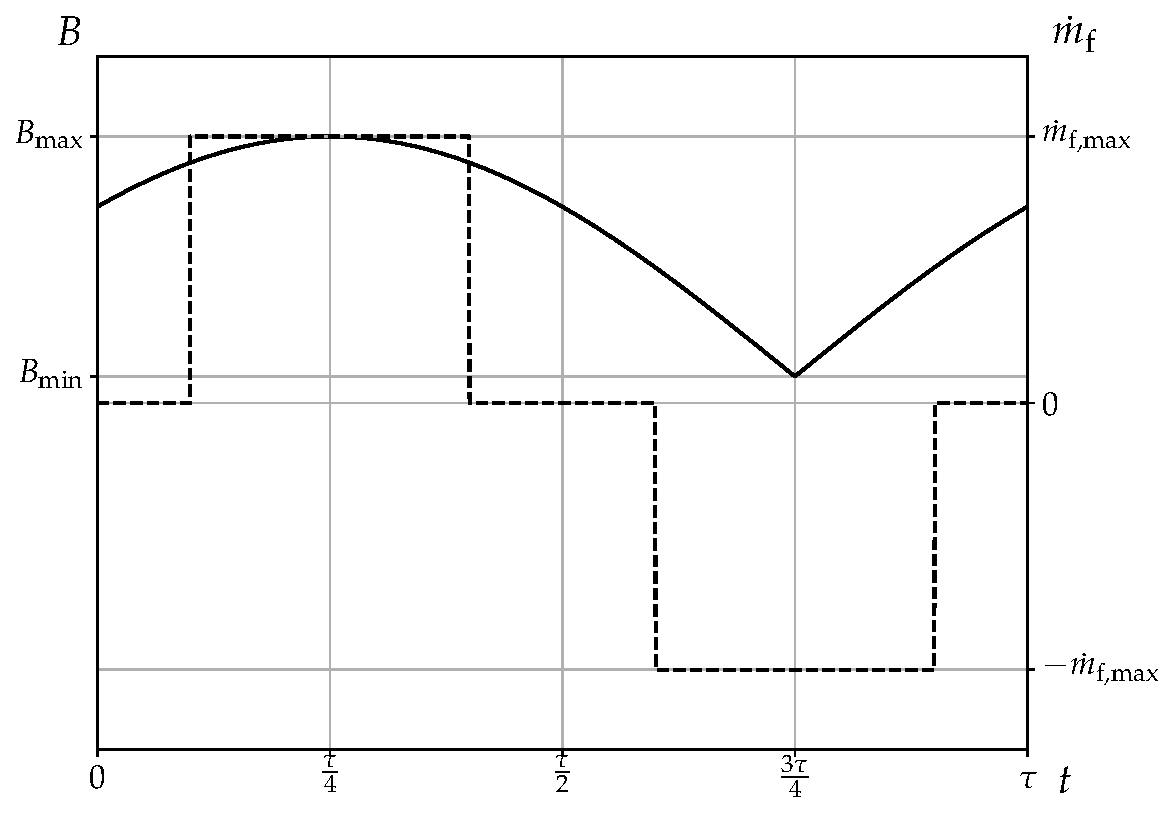
\includegraphics[width=7cm]{profiles_rc_and_flow_instantaneous}
  \caption{Rectified cosine magnetic profile and the instantaneous flow profile with blow fraction of \SI{60}{\percent}}
  \label{fig:cos-inst-60}
\end{figure}

Figure~\ref{fig:cos_ins} shows the cooling capacity attained by the device at a frequency of \SI{1}{\hertz} and different utilizations, for both comparison methods. The horizontal axis shows the average value during the high field region. 
\textcolor{black}{For} Fig.~\ref{fig:comp_min}, the instantaneous profile almost always yields a higher performance, while for Fig.~\ref{fig:comp_avg} the rectified cosine profile generates higher cooling capacities. Since the average \textcolor{black}{field} during the hot cycle (high field stage) is the same, the main difference is due to the low magnetic field levels. For the ``same minimum'' comparison, the instantaneous profile is capable of keeping the magnetic field at low levels for the whole half-cycle, which is beneficial for performance;  for $\Phi=1.0$ and $\average{B}\ped{high} = \SI{1.40}{\tesla}$, the cooling capacity for the instantaneous profile is $\SI{196.3}{\percent}$ higher than for the cosine profile.  As demonstrated by \cite{bib:asme-mce}, a higher average magnetic field during the low-field stage increases the solid temperature and consequently results in  warmer fluid entering the cold heat exchanger, representing a thermal loss. In the ``same-average'' comparison, the cosine profile is capable of achieving much lower levels (since its minimum value is fixed), therefore providing more cooling power. However, as explained before, this \textcolor{black}{analysis serves mainly the purpose of illustrating the influence of low magnetic field variation, by looking at two hypothetical scenarios. More} complex \textcolor{black}{magnetic circuit}  geometries \textcolor{black}{are} required to generate the instantaneous magnetic profile \textcolor{black}{with a} low \textcolor{black}{magnetic field} close to 0.


\begin{figure}[!ht]
  \centering
  \subfloat[Same minimum]{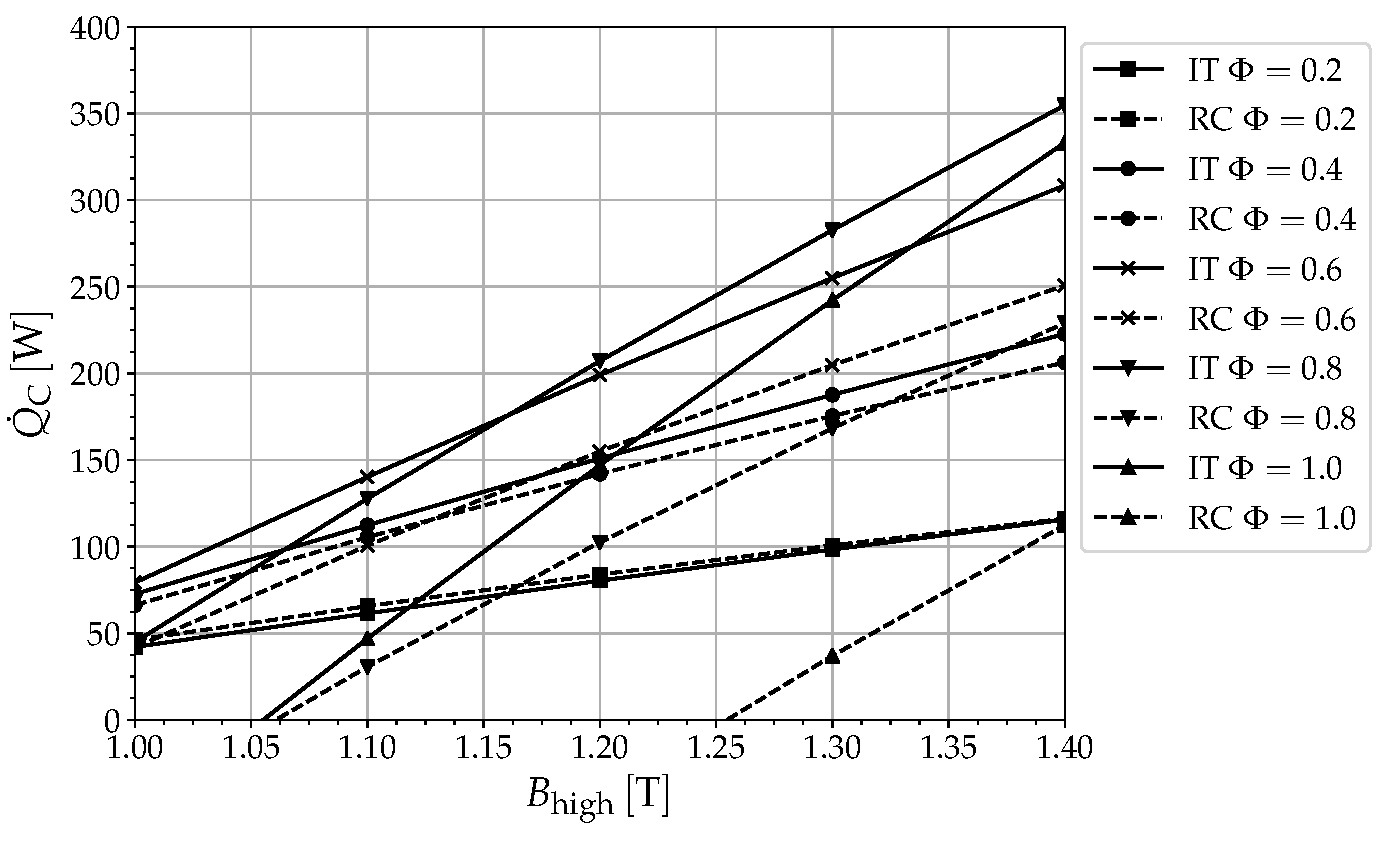
\includegraphics[width=8cm]{Qc_B_comp_f_1_same_minimum}\label{fig:comp_min}}
\,
%  \subfloat[Same average]{\includegraphics[width=8cm]{Qc_B_comp_f_1_same_low_average}\label{fig:comp_avg}}
\,
  \caption{Cooling capacity as a function of the  average high magnetic field, for different utilizations. \textcolor{black}{``IT''}: instantaneous (blow fraction of \SI{100}{\percent}); ``RC'': rectified cosine  (blow fraction of \SI{60}{\percent}), for both comparison methods.}
 \label{fig:cos_ins}
\end{figure}

The only exception in the ``same minimum'' comparison is seen for the lowest utilization of $\Phi = 0.2$, where the performance is slightly better for the RC profile. Since the blow fraction for the cosine is lower, the mass flow rate \textcolor{black}{is} higher \textcolor{black}{in the latter for} the same utilization (cf. Eq.~\eqref{eq:200}). \textcolor{black}{This} increases \textcolor{black}{the} heat transfer rate, as previously explained ---  outweighing the effects of the magnetic field.


The same analysis, but in terms of the coeficient of performance, is shown in \autoref{fig:cos_ins_cop}. For the ``same average'' analysis, the $\cop$ results show the same trends as the cooling capacity. However, for the \textcolor{black}{somewhat} more realistic analysis where the minimum of both profiles are the same, the rectified cosine profile yields better results for small values of utilization. This is due to \textcolor{black}{a} lower pumping power, as the mass flow rate for the cosine profile is slightly higher, but also flows for a shorter period of time. \textcolor{black}{Since} in this region the cooling capacity for the RC profile can be close to or higher than the \textcolor{black}{IT} profile (cf. Fig.~\autoref{fig:comp_min}), the coefficient of performance becomes higher for the rectified cosine profile.

\begin{figure}[!ht]
  \centering
  \subfloat[Same minimum]{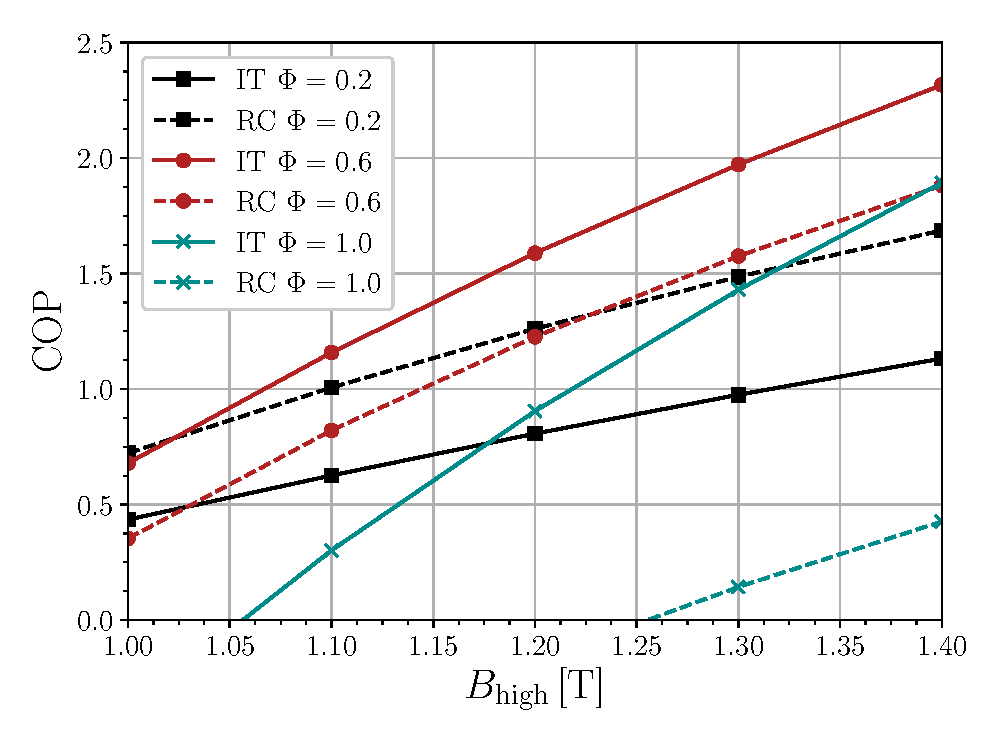
\includegraphics[width=7cm]{COP_B_comp_f_1_same_minimum}\label{fig:comp_min_cop}}
\,
%  \subfloat[Same average]{\includegraphics[width=7cm]{COP_B_comp_f_1_same_low_average}\label{fig:comp_avg_cop}}
\,
  \caption{Coefficient of performance as a function of the  average high magnetic field, for different utilizations. \textcolor{black}{``IT''}: instantaneous (blow fraction of \SI{100}{\percent}); ``RC'': rectified cosine  (blow fraction of \SI{60}{\percent}), for both comparison methods.}
 \label{fig:cos_ins_cop}
\end{figure}

In general, considering the goal of achieving target requirements for the cooling capacity, AMRs operating with the instantaneous magnetic profile \textcolor{black}{generate} better \textcolor{black}{performance} results. As can be seen \textcolor{black}{in} Fig.~\ref{fig:cos_ins}, an instantaneous profile with the lowest possible value of $B\ped{min}$ and the highest possible value of $B\ped{max}$, with a flow profile occupying the whole cycle with average values of utilization, results in the highest values of cooling capacity among all simulations. 

The rectified cosine profile, found in compact systems using Halbach arrays, can \textcolor{black}{surely} benefit from reducing the blow fraction, both in terms of cooling capacity and temperature span. However, for the typical parameters \textcolor{black}{evaluated} in this Thesis, even if the blow fraction is optimized for the ``RC'' profile, the ``IT'' profile still yields better results.

\subsubsection{Analysis of the instantaneous profile}
\label{sec:deta-analys-inst}

As shown in the previous section, the instantaneous profile \textcolor{black}{generally} yields the highest values \textcolor{black}{of} cooling capacity. Therefore, in this section, a more detailed analysis of \textcolor{black}{this} profile has been carried out, \textcolor{black}{where the} maximum field in \autoref{fig:cobem-profiles} \textcolor{black}{is} varied, while the minimum value is kept at \SI{0.05}{\tesla}. Figure~\ref{fig:qc_phi_inst} shows the cooling capacity as a function of \textcolor{black}{the} utilization, for several levels of the maximum magnetic field \textcolor{black}{and} two different operating frequencies. Because of the conflict between a low heat transfer rate for flow rates \textcolor{black}{that are} too low and losses in regenerator effectiveness in flow rates \textcolor{black}{that are} too high, there are critical values of utilization that maximize \textcolor{black}{the} cooling capacity, and this critical values increases with the magnetic field. \textcolor{black}{For} higher magnetic fields, the increase in the MCE surpasses the loss of effectiveness, and one can go to higher flow rates without losing performance. It can also be seen in Fig.~\ref{fig:qc_phi_inst} that at  higher frequencies the values of cooling power are higher, and also the critical values of utilization are lower; however, this \textcolor{black}{is} usually achieved at the \textcolor{black}{expense} of \textcolor{black}{a} higher power consumption in AMR devices at higher frequencies \cite{bib:lei15_study,NIKNIA2016601}.

\begin{figure}[!ht]
  \centering
\subfloat[$f = \SI{1}{\hertz}$]{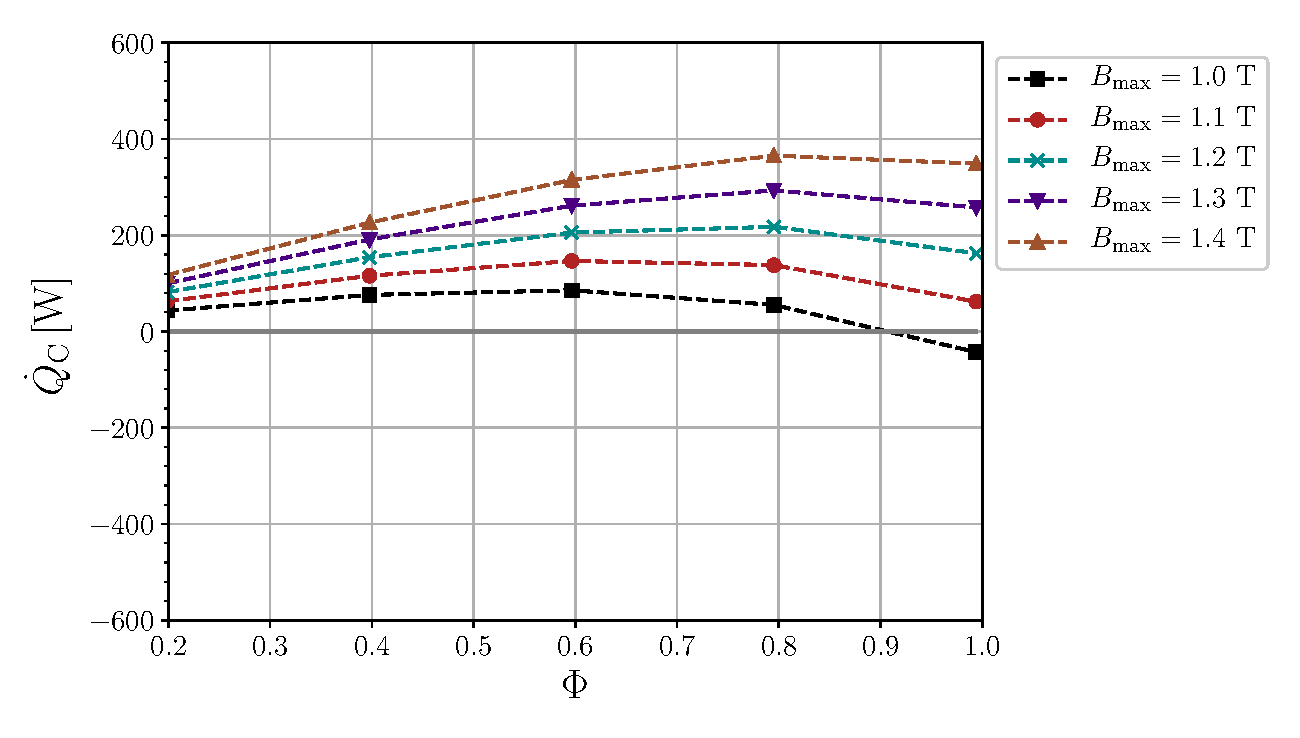
\includegraphics[width=8cm]{Qc_Phi_inst_f_1_Hmin_005_FB_100}\label{fig:Qc_phi_inst_1}}
\,
  \subfloat[$f = \SI{2}{\hertz}$]{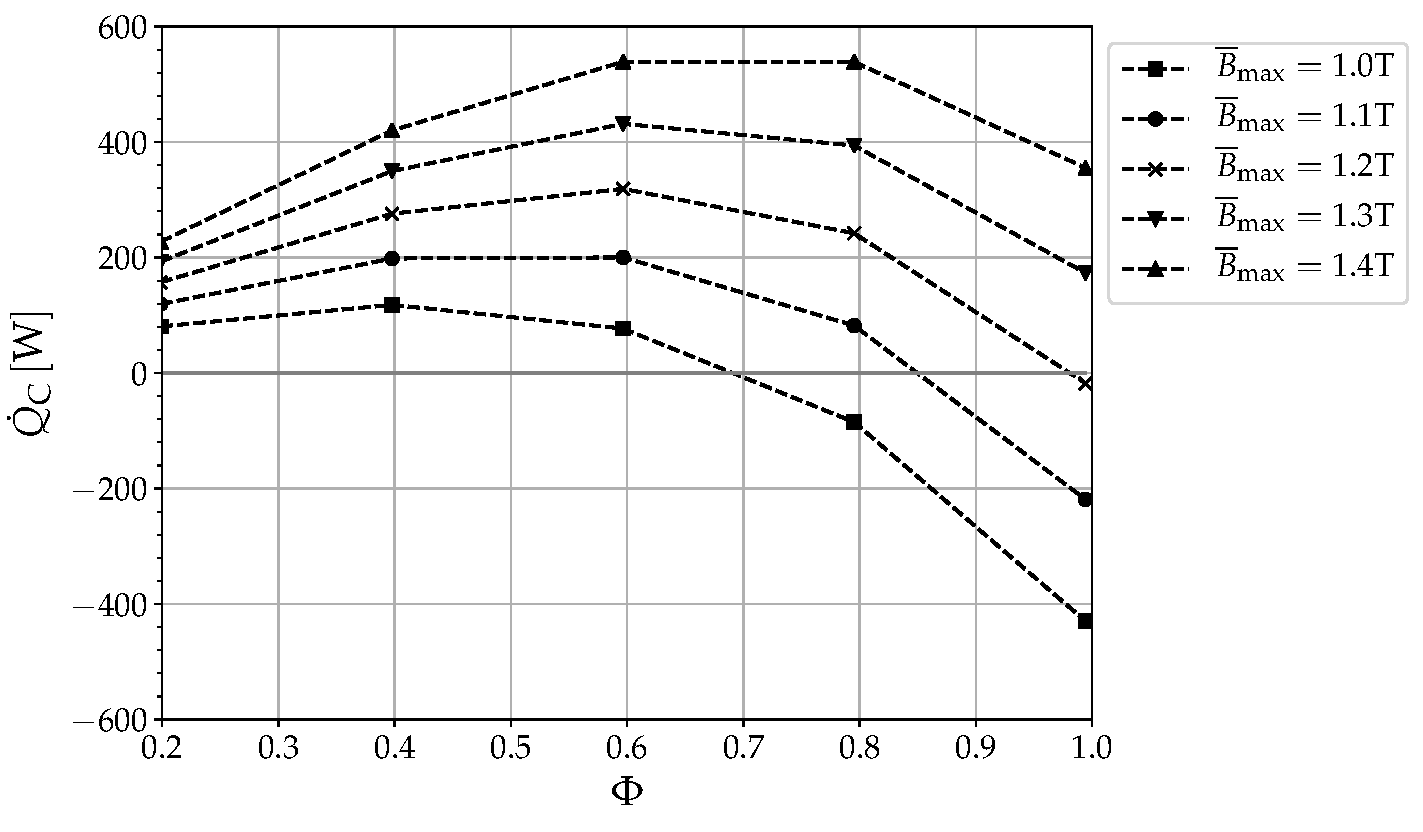
\includegraphics[width=8cm]{Qc_Phi_inst_f_2_Hmin_005_FB_100}\label{fig:Qc_phi_inst_2}}
  \caption{Cooling capacity as a function of utilization, for various values of the high magnetic field  \textcolor{black}{for} the instantaneous profile}
  \label{fig:qc_phi_inst}
\end{figure}

\begin{figure}[!ht]
  \centering
  \subfloat[Cooling capacity]{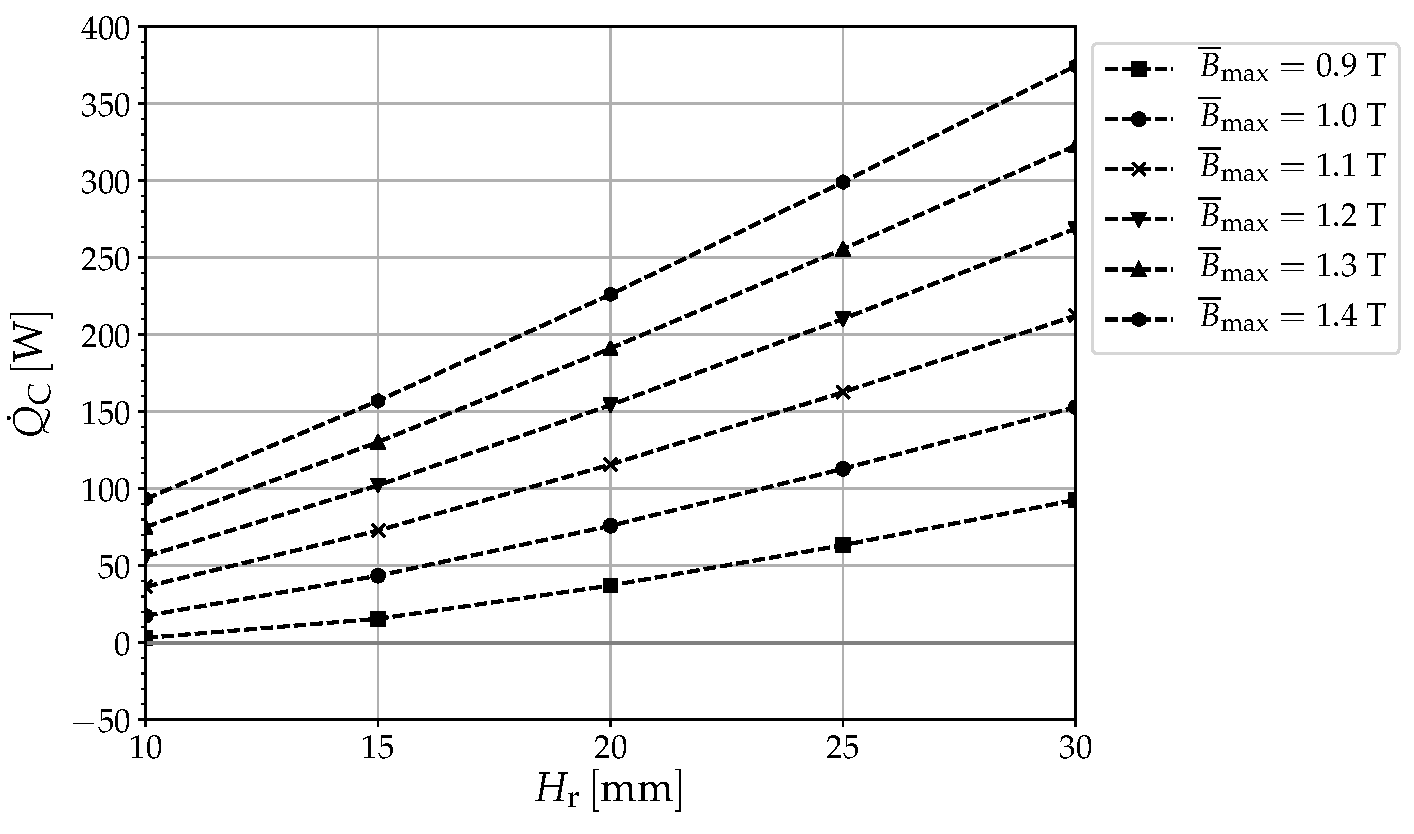
\includegraphics[width=9cm]{Qc_H_inst_f_1_Phi_40}\label{fig:Qc_H_inst_f_1_Phi_40}}
\quad
  \subfloat[Coefficient of performance]{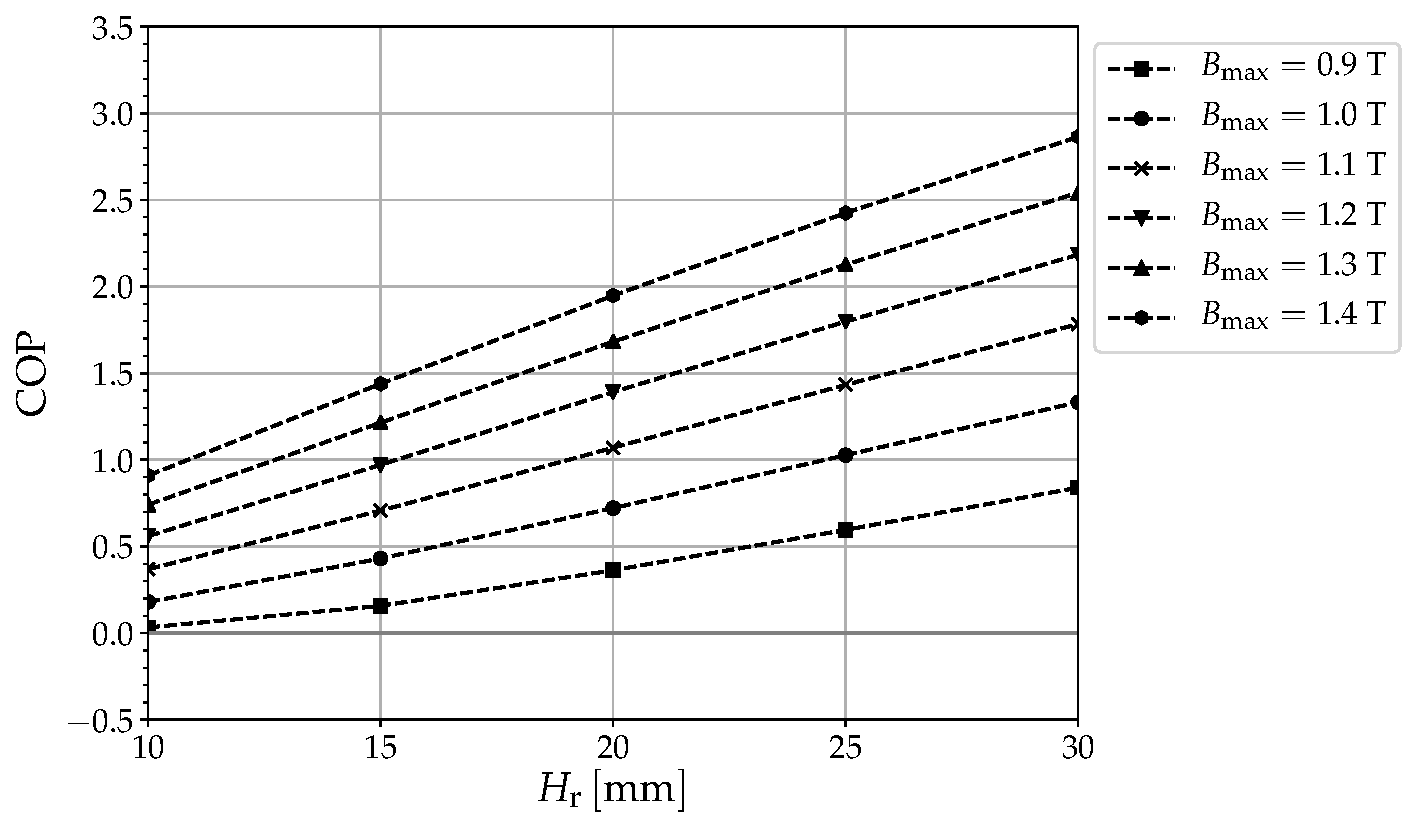
\includegraphics[width=9cm]{COP_H_inst_f_1_Phi_40}\label{fig:COP_H_inst_f_1_Phi_40}}
  \caption{Performance metrics as a function of \textcolor{black}{the} regenerator height (all other parameters \textcolor{black}{were set as in} Table~\ref{tab:params-cobem}, \textcolor{black}{for}  utilization factor of 0.4) for various values of the high magnetic field of the instantaneous profile}
\label{fig:Qc_H_inst}
\end{figure}

The parameters in \autoref{tab:params-cobem} were chosen from preliminary simulations, \textcolor{black}{so} they are not  optimal. To understand the impact of \textcolor{black}{the} regenerator geometry on the performance with the instantaneous profile, the regenerator height was varied in Fig.~\ref{fig:Qc_H_inst}, and all other parameters from \autoref{tab:params-cobem} were kept fixed and with $\phi=0.4$. As expected, higher magnetic fields allow for smaller regenerators (hence more compact systems) to achieve a \textcolor{black}{desired} cooling capacity. For instance, to achieve a capacity of \SI{100}{\watt}, increasing the field from \num{1.0} to \SI{1.2}{\tesla} \textcolor{black}{results} in regenerators \textcolor{black}{that are} \SI{36}{\percent} smaller. Comparing results \textcolor{black}{for} cooling capacity and coefficient of performance, the trends are largely the same, as the former is more sensitive to variations in the magnetic field and regenerator height than the components of power.


\subsection{In-depth analysis of the  magnetic \textcolor{black}{ramp} profile}
\label{sec:performance-an-amr-1}

Based on the better performance of the instantaneous profile, the ramp profile is assumed as a suitable target profile for the design of magnetic refrigerators, and will be analyzed in this section.

Moving towards a more realistic model, casing losses are included, using the model from \cite{bib:trevizoli16_perfor_model}. The bed is enclosed in a solid casing of thickness $h\ped{csg}$, and two air layers of thickness $h\ped{air}$ separate \textcolor{black}{the AMR and its casing} from the inner and outer \textcolor{black}{magnet} cylinders. 

\begin{figure}[!ht]
  \centering
  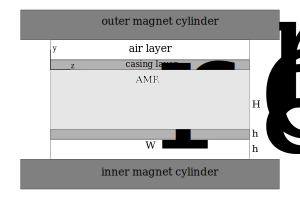
\includegraphics[width=7cm]{amr-casing}
  \caption{Model for the casing losses in regenerators}
  \label{fig:amr-casing}
\end{figure}

\nomenclature[ia]{air}{air layer between magnets and regenerators}
\nomenclature[ic]{csg}{regenerator casing}

Preliminary analyses \textcolor{black}{carried out by} \cite{bib:peixer17-perfor-amrs} using the losses model described in \autoref{sec:model-casing-loss} showed that a stainless steel casing \textcolor{black}{with a} thickness \textcolor{black}{of} $h\ped{csg} = \SI{0.5}{\mm}$ is thick enough to ensure mechanical integrity and easy manufacturing, while being thin enough to accommodate the material \textcolor{black}{with a low} thermal conductivity. 

In addition, \textcolor{black}{in the present study}, an air gap clearance thickness was set at $h\ped{air} = \SI{1}{\mm}$. This value \textcolor{black}{gave rise to a} peak in cooling capacity due to the compromise between minimizing losses and maximizing the magnetocaloric mass.

The simulations in this section also use multilayer regenerators. A summary of all parameters adopted in this section, including the Curie temperatures and volumetric fractions (relative to the length of the bed) of each layer is presented in \autoref{tab:params-ramp}.

\begin{table}[!ht]
  \centering
  \begin{tabular}{c|c}
\hline
    \textbf{Parameter} & \textbf{Value} \\
\hline
$R\ped{o}$ & \SI{40}{\mm} \\
$W\ped{r}$ & \SI{30}{\mm} \\
$L\ped{r}$ & \SI{85}{\mm} \\
$N\ped{r}$ & \num{8} \\
$N\ped{v}$ & \num{16} \\
$f$ & \SI{1}{\hertz} \\
$\th$ & \SI{305.5}{\kelvin} = \SI{32.5}{\celsius} \\
$\tc$ & \SI{270.5}{\kelvin} = \SI{-2.5}{\celsius} \\
$D\ped{p}$ & \SI{350}{\micro\meter} \\
$h\ped{csg}$ & \SI{0.5}{\mm} \\
$h\ped{air}$ & \SI{1}{\mm} \\
Casing material & Stainless steel \\
Number of layers & \num{3} \\
Curie temperatures of each layer & \num{273}, \num{283}, \SI{290}{\kelvin} \\ 
Length fractions of each layer & \num{20}, \num{20}, \SI{60}{\percent}\\
\hline
  \end{tabular}
  \caption{Fixed parameters for the AMR simulations used in this chapter}
  \label{tab:params-ramp}
\end{table}


\subsubsection{Synchronization between \textcolor{black}{the} fluid flow and magnetic profiles}
\label{sec:synchr-betw-fluid}

A central point of this Thesis is \textcolor{black}{related to} the importance of two characteristic waveforms, the fluid flow and magnetic profiles, \textcolor{black}{and how they affect} the performance of a magnetic refrigerator. Several works have independently investigated the synchronization between these profiles \cite{bib:bjoerk11_amr,bib:nakashima17-exper}. Here, \textcolor{black}{the} focus is  on the parameterization of these waveforms and \textcolor{black}{the} characerization of an AMR system with these parameters, in particular the blow fraction (cf. \autoref{sec:inst-fluid-flow}) and the magnetization fraction (cf. \autoref{sec:ramp-magn-prof}). Figure~\ref{fig:ramp-inst} shows the two profiles that will be used in this section.

\begin{figure}[!ht]
  \centering
  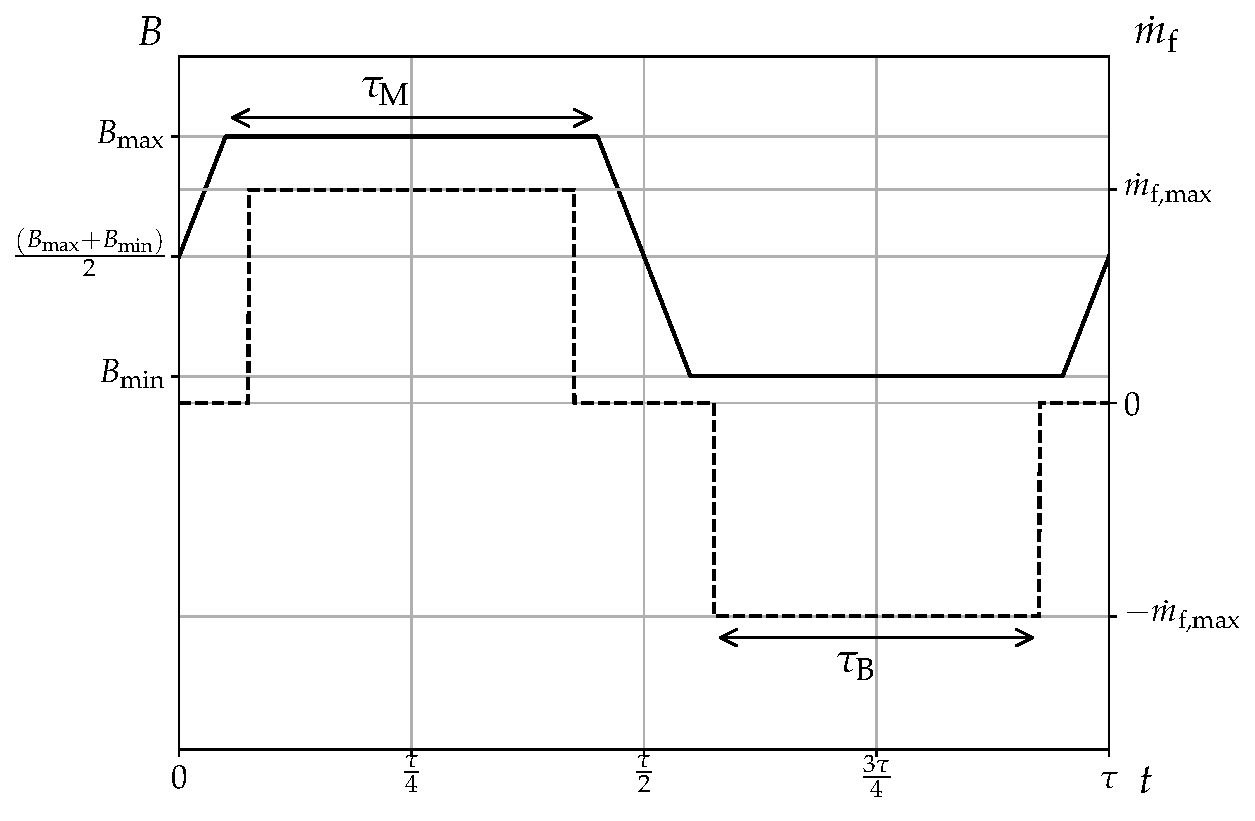
\includegraphics[width=7cm]{profiles_rm_and_flow_instantaneous}
  \caption{Comparison between the magnetic \textcolor{black}{ramp} profile (solid line) and the instantaneous fluid flow profile (dashed line)}
  \label{fig:ramp-inst}
\end{figure}
 

Regarding the magnetic profile, the \textcolor{black}{magnitude of the} high value will be varied to investigate the performance of the AMR system, while the minimum will be kept at $\bmin = \SI{0.05}{\tesla}$. Ideally, this value \textcolor{black}{should be nil}, but it is \textcolor{black}{difficult} to achieve complete flux insulation in the low field region, so \textcolor{black}{a finite value of the} minimum field is \textcolor{black}{adopted}.

\subsubsection{Performance curves for varying blow and magnetization fractions}
\label{sec:perf-curv-vary}

Figure~\ref{fig:Qc_COP_curves_phi40} shows the cooling capacity and coefficient of performance of the AMR system for a fixed utilization factor of \num{0.4} and for a magnetic profile with \textcolor{black}{a} maximum at \SI{1.3}{\tesla}, for \textcolor{black}{variable} blow and magnetization fractions. \textcolor{black}{To facilitate the analysis, the} results are plotted in terms of the ratio $\nicefrac{F\ped{M}}{F\ped{B}}$, with curves for different \textcolor{black}{values of} $F\ped{B}$. It is clear \textcolor{black}{that both the cooling capacity and the coefficient of performance exhibit a peak at} $F\ped{M} = F\ped{B}$. Moreover,  \textcolor{black}{to the right of the peak, i.e., for higher values of $F\ped{M}$, the}  reduction \textcolor{black}{of} both \textcolor{black}{performance} metrics \textcolor{black}{is} slower, meaning it is better to have a magnetization plateau wider than the fluid flow plateau, thus confirming the conclusions \textcolor{black}{of} \autoref{cha:exper-invest-fluid}. 

The reduction in performance for $F\ped{M} > F\ped{B}$ \textcolor{black}{can be explained by an increase in} heat leakage through the casing, as the solid begins to lose energy to the environment \textcolor{black}{when} the fluid is not flowing. For $F\ped{M} < F\ped{B}$, the effect \textcolor{black}{discussed in} \autoref{sec:results-discussions} is present: the fluid begins to flow when the solid is not totally warmed up, losing effectiveness.

\begin{figure}[!ht]
  \centering
  \subfloat[Cooling capacity]{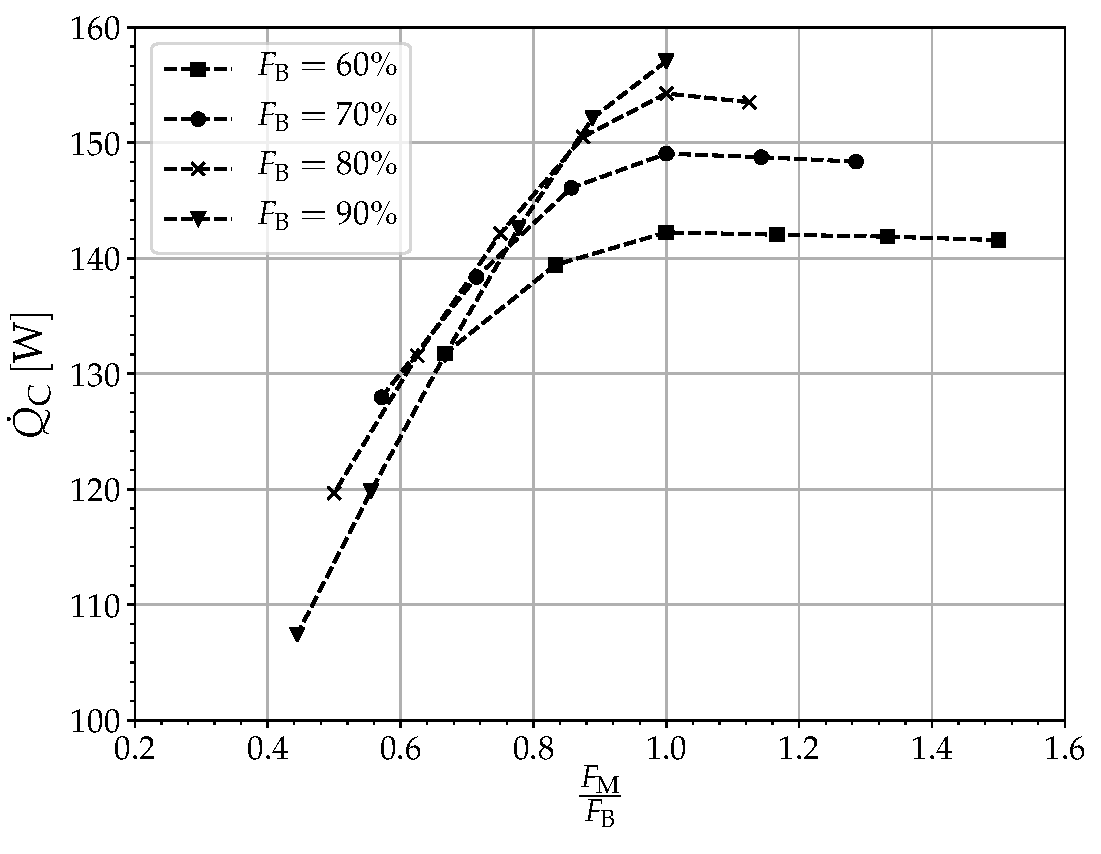
\includegraphics[width=5cm]{Qc_FM_ramp_f_1_Phi_40_35K_1300mT}\label{fig:Qc_FM_ramp_f_1_Phi_40_35K_1.3T}}
\quad
 \subfloat[Coefficient of performance]{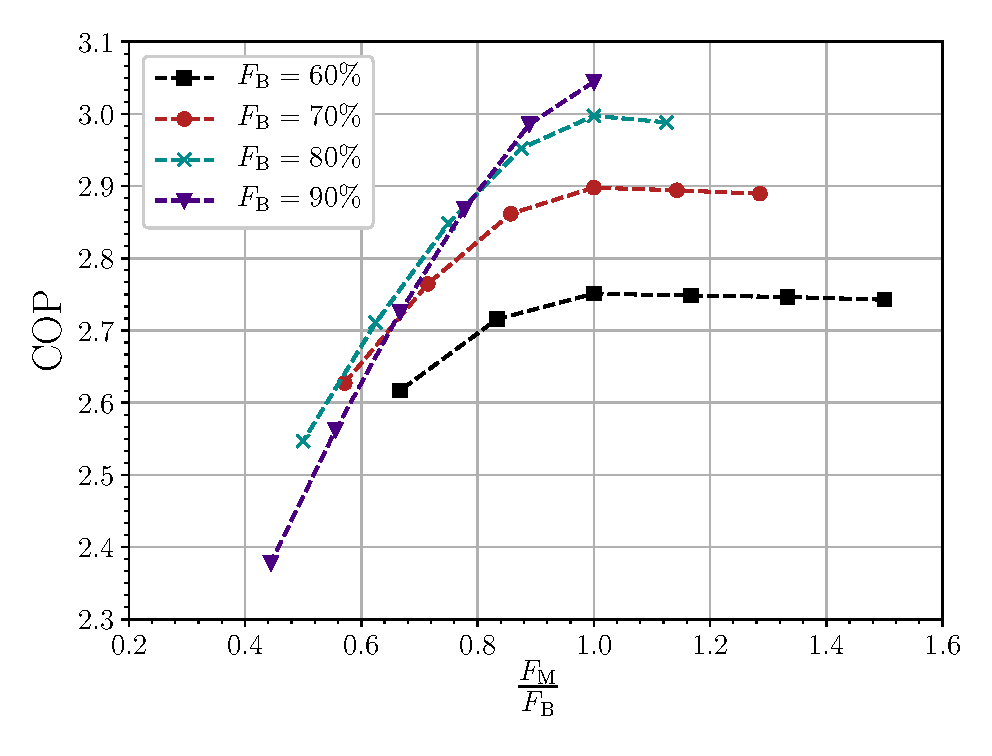
\includegraphics[width=5cm]{COP_FM_ramp_f_1_Phi_40_35K_1300mT}\label{fig:COP_FM_ramp_f_1_Phi_40_35K_1.3T}}
  \caption{Performance of the AMR system for various blow and magnetization fractions, utilization of 0.4 and and high magnetic field of \SI{1.3}{\tesla}}
  \label{fig:Qc_COP_curves_phi40}
\end{figure}

The influence of \textcolor{black}{the} utilization is demonstrated in \autoref{fig:Qc_curves_ramp_phi}, where the cooling capacity \textcolor{black}{is} plotted for different utilization factors. For increasing $\Phi$ in this range, not only do the overall values of cooling capacity increase, but also the importance of choosing the blow fraction becomes clearer. In \textcolor{black}{these ranges} of utilization and blow fraction,  the cooling capacity increases because the higher transfer rate associated with higher flow rates \textcolor{black}{dominates} over the loss of regenerator effectiveness.

\begin{figure}[!ht]
  \centering
  \subfloat[$\Phi = \num{0.2}$]{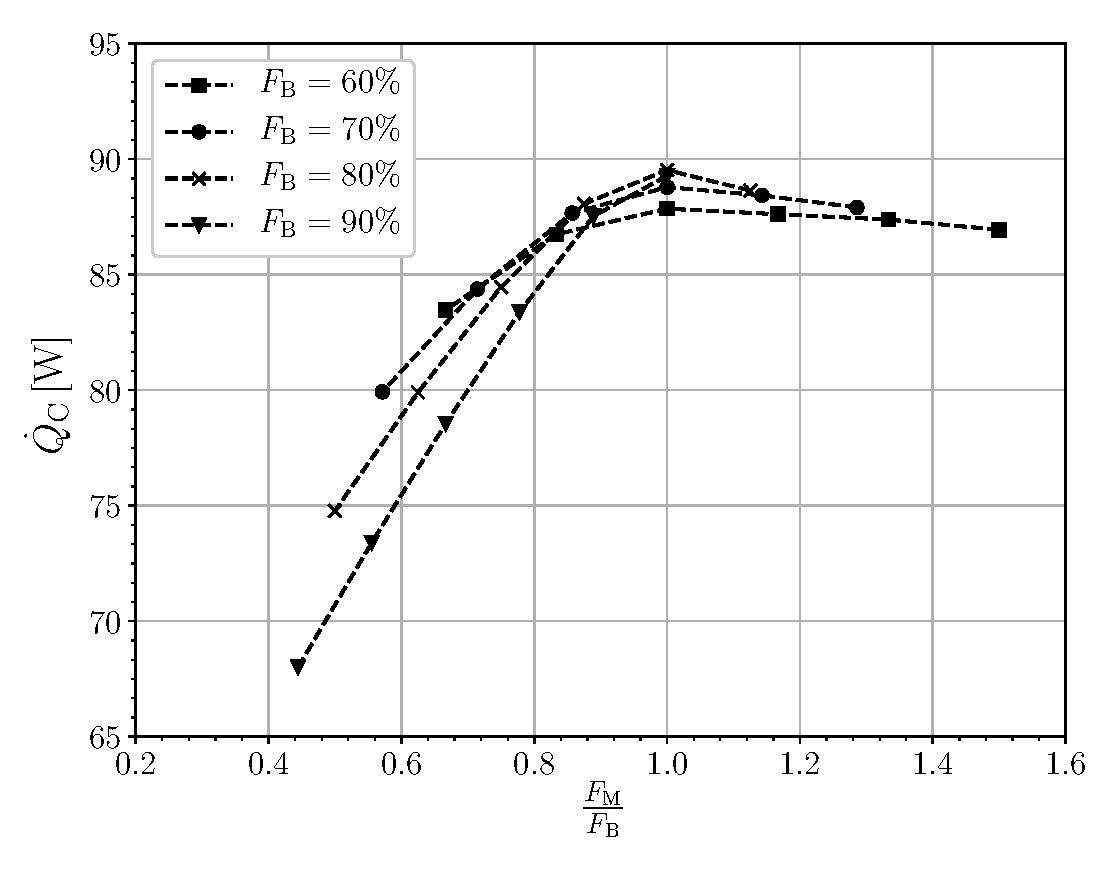
\includegraphics[width=5cm]{Qc_FM_ramp_f_1_Phi_20_35K_1300mT}\label{fig:Qc_FM_ramp_f_1_Phi_20_35K_1.3T}}
\quad
 \subfloat[$\Phi = \num{
0.5}$]{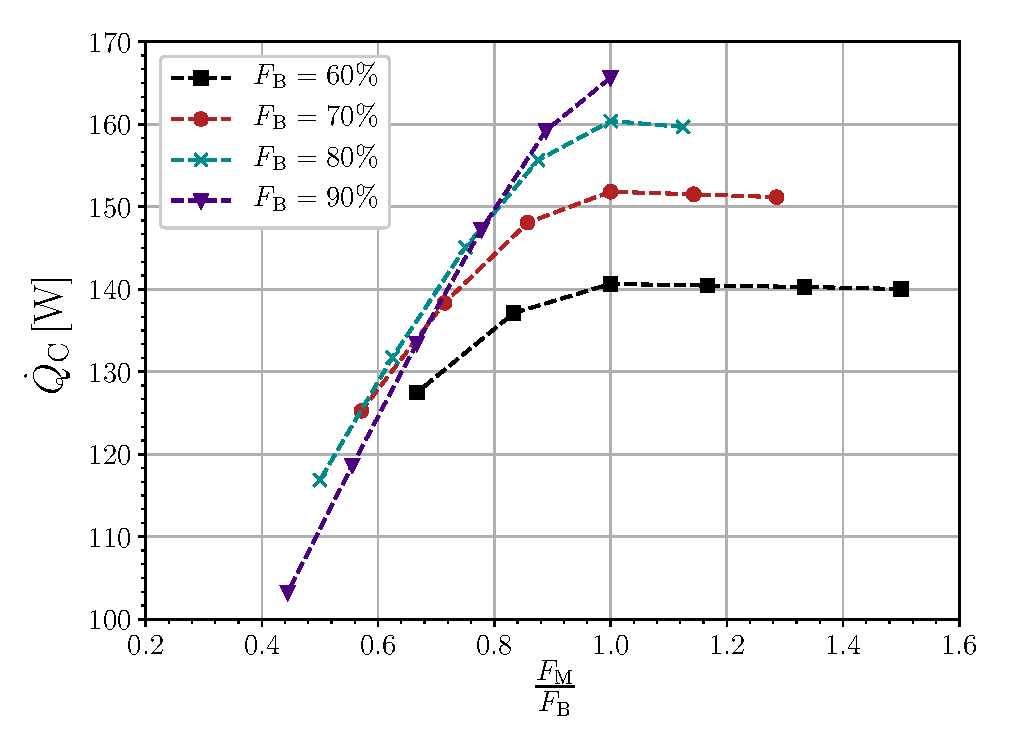
\includegraphics[width=5cm]{Qc_FM_ramp_f_1_Phi_50_35K_1300mT}\label{fig:COP_FM_ramp_f_1_Phi_50_35K_1.3T}}
  \caption{Influence of utilization on the cooling capacity of the AMR system for  various blow and magnetization fractions, with high magnetic field of \SI{1.3}{\tesla}}
  \label{fig:Qc_curves_ramp_phi}
\end{figure}

The \textcolor{black}{above} results can be \textcolor{black}{evaluated from} another point of view with \autoref{fig:COP_maps_ramp_FM}, where the coefficient of performance is plotted as contour levels. This type of map is useful because, since $\bmin$ and $\tau$ are fixed, each point in this graph completely characterizes a magnetic \textcolor{black}{ramp} profile, and each subplot with fixed $\Phi$ and $F\ped{B}$ characterizes the fluid flow profile. As expected, the performance increases for the higher values both $\bmax$ and $F\ped{M}$, where the  magnetic \textcolor{black}{ramp} profile tends to the instantaneous magnetic profile with a large amplitude. Confirming the previous trends, the results are less sensitive to the magnetization fraction when $F\ped{M} \ge F\ped{B}$. 

\begin{figure}[!ht]
  \centering
  \subfloat[$\Phi = 0.2, F\ped{B} = \SI{60}{\percent}$]{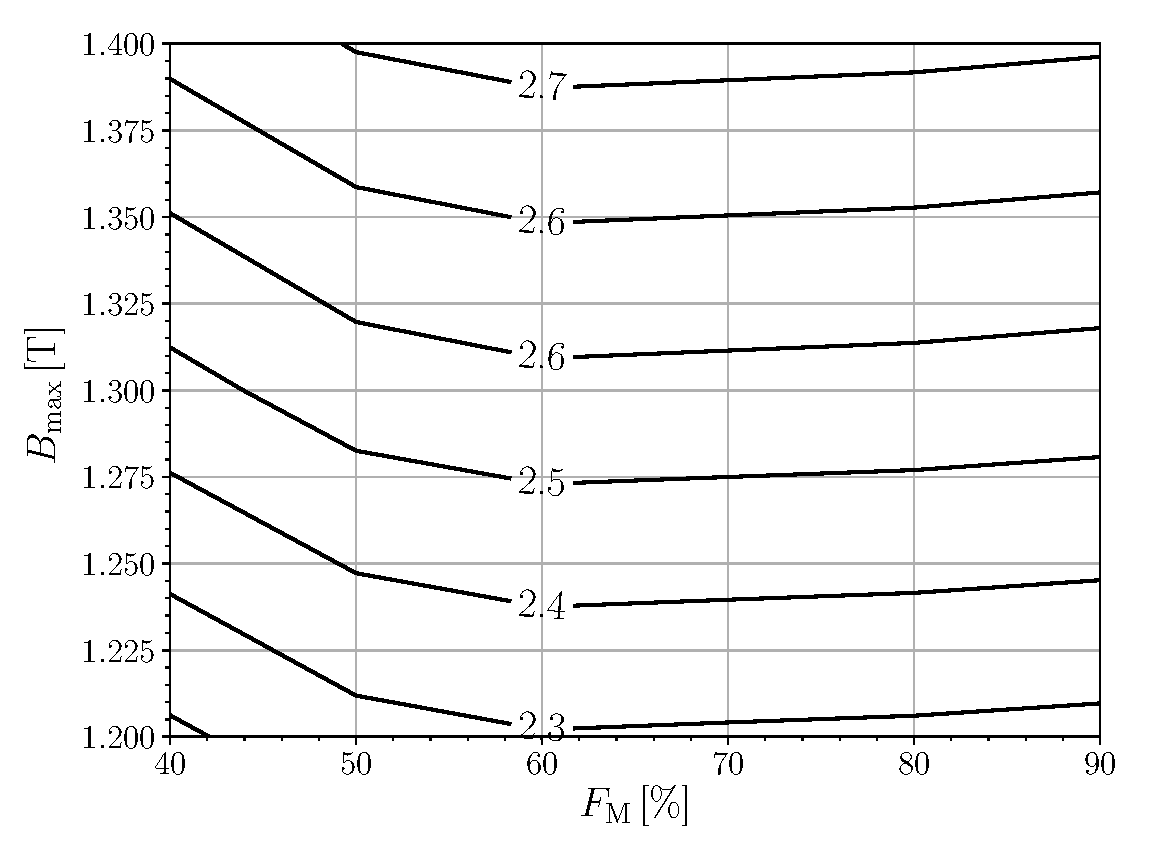
\includegraphics[width=5cm]{COP_ramp_map_f_1_Phi_20_FB_60_35K_Valv_ASCO}\label{fig:COP_ramp_map_f_1_Phi_20_FB_70_35K_Valv_ASCO}}
\quad
 \subfloat[$\Phi= 0.2, F\ped{B} = \SI{90}{\percent}$]{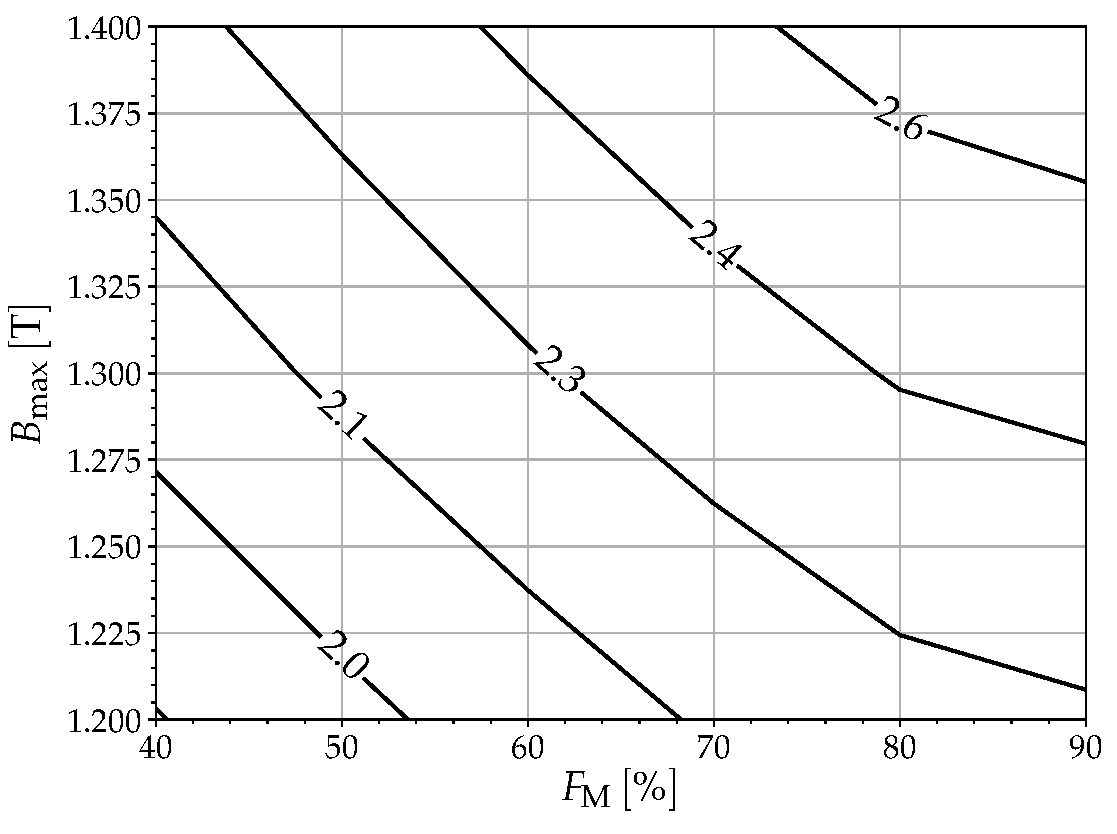
\includegraphics[width=5cm]{COP_ramp_map_f_1_Phi_20_FB_90_35K_Valv_ASCO}\label{fig:COP_ramp_map_f_1_Phi_20_FB_90_35K_Valv_ASCO}} \\
  \subfloat[$\Phi = 0.4, F\ped{B} = \SI{60}{\percent}$]{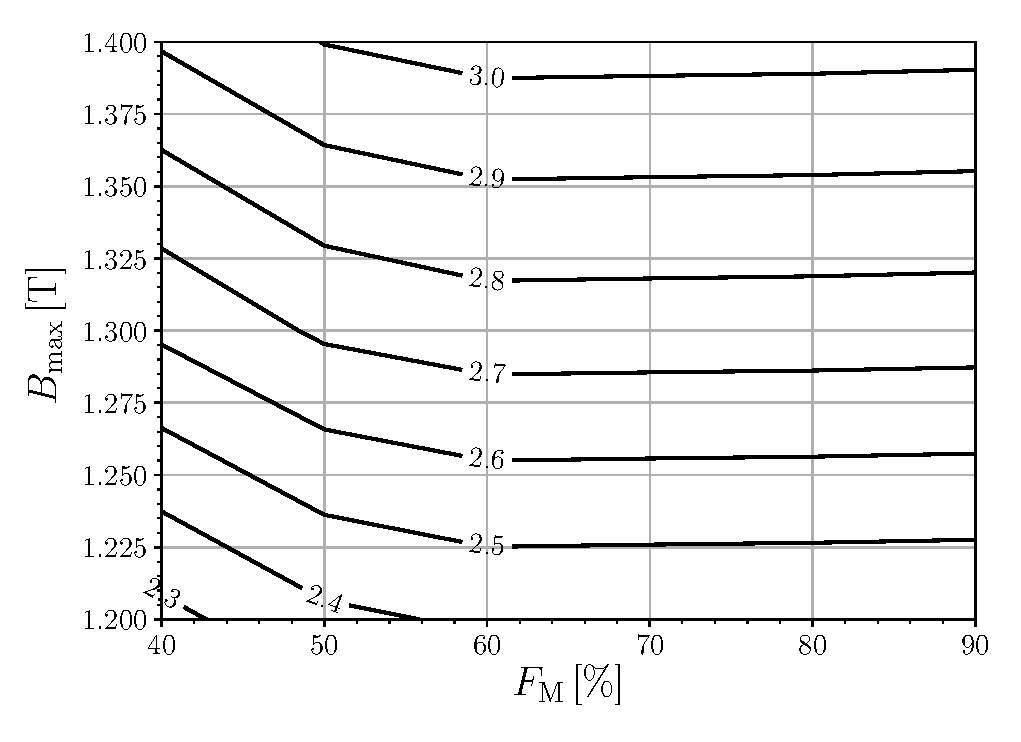
\includegraphics[width=5cm]{COP_ramp_map_f_1_Phi_40_FB_60_35K_Valv_ASCO}\label{fig:COP_ramp_map_f_1_Phi_60_FB_90_35K_Valv_ASCO}}
\quad
 \subfloat[$\Phi = 0.4, F\ped{B} = \SI{90}{\percent}$]{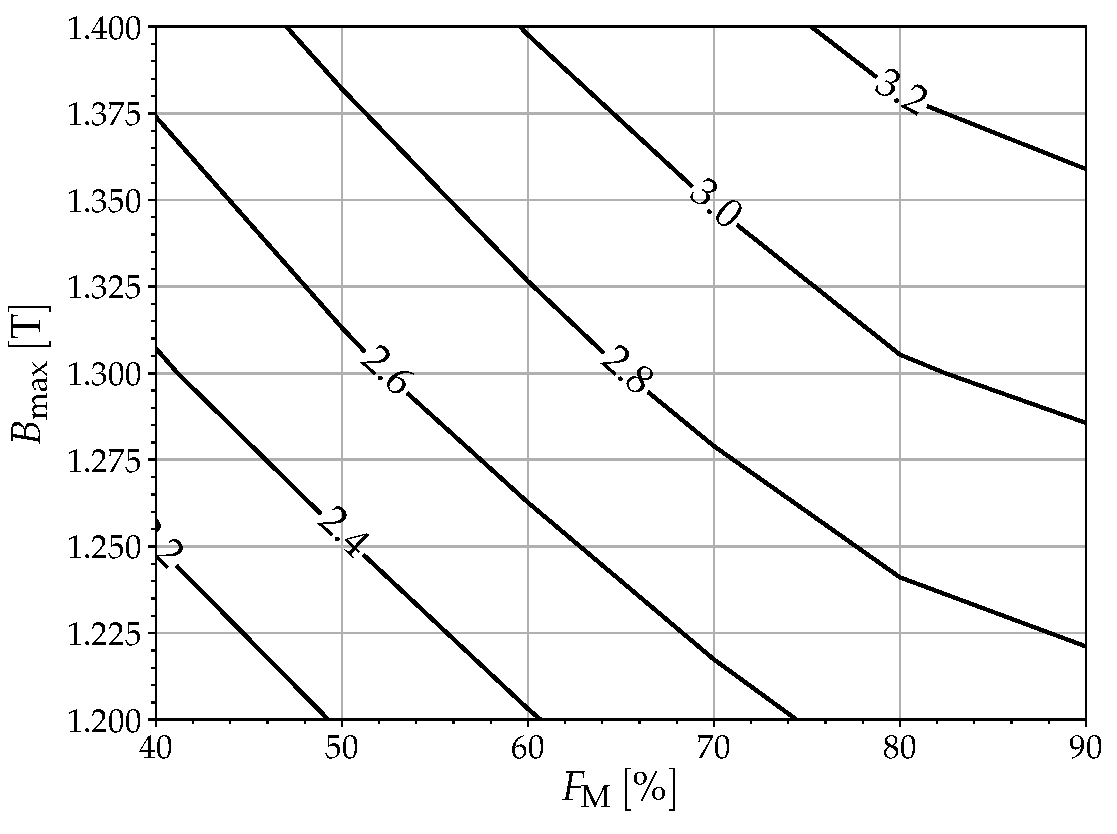
\includegraphics[width=5cm]{COP_ramp_map_f_1_Phi_40_FB_90_35K_Valv_ASCO}\label{fig:COP_ramp_map_f_1_Phi_40_FB_90_35K_Valv_ASCO}}
  \caption{Influence of utilization and blow fraction on the coefficient of performance of the AMR system for varying high magnetic field and magnetization fraction}
  \label{fig:COP_maps_ramp_FM}
\end{figure}

\subsubsection{Geometric analysis of the regenerators using the ramp magnetic profile}
\label{sec:geom-analys-regen}

\textcolor{black}{All} previous results assumed a fixed regenerator geometry, with the goal of identifying the optimal fluid and magnetic profile parameters. \textcolor{black}{It became clear that the} magnetization fraction should be as large as possible, but that makes it more difficult to design a magnetic circuit \textcolor{black}{based on} permanent magnets. The value of $F\ped{M} = \SI{70}{\percent}$ is then chosen as a compromise, with \textcolor{black}{a corresponding} $F\ped{B} = F\ped{M}$. The mean value of \textcolor{black}{the} utilization factor of $\Phi = 0.4$ is also chosen as reference in the next results.

In this section, the \textcolor{black}{effect of the} regenerator height is \textcolor{black}{evaluated. The results will complement those for the} air gap height that will be shown in \autoref{cha:design-optim-magn} concerning the design of the magnetic circuit. The importance of the air gap height as a coupling \textcolor{black}{parameter} between the geometric design of the regenerators and the magnetic circuit was explored using a simplified model in \autoref{sec:performance-an-amr} and using the instantaneous magnetic profile in \autoref{sec:deta-analys-inst}. The results \textcolor{black}{to be} shown \textcolor{black}{here} use the magnetic \textcolor{black}{ramp} profile \textcolor{black}{studied in depth in} this present chapter.

Figure~\ref{fig:qc-cop-eta-amr-height} shows the cooling capacity, coefficient of performance and second-law efficiency for varying magnetic field and regenerator height. \textcolor{black}{As} expected, larger regenerators can \textcolor{black}{produce} the desired performance with lower magnetic fields. It can also be seen that this configuration for an AMR system can achieve values of $\etasec$ compatible with conventional vapor compression systems \cite{HERMES20081341,NEGRAO20113051}, although these numerical results do not include mechanical losses.

\begin{figure}[!ht]
  \centering
\subfloat[Cooling capacity (solid lines) and coefficient of performance (dashed lines)]{  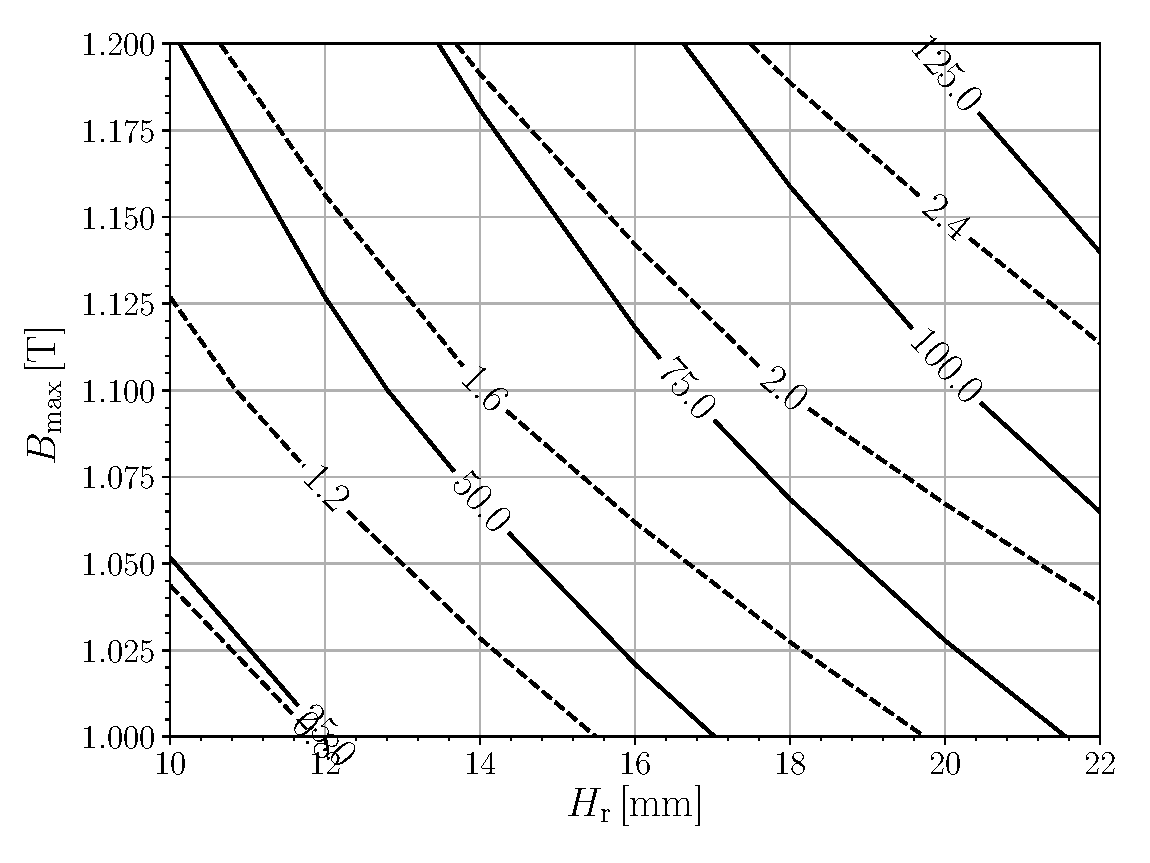
\includegraphics[width=5cm]{Qc_COP_combined_H_regW30}\label{fig:Qc_COP_Hreg}}
\,
\subfloat[Second-law efficiency]{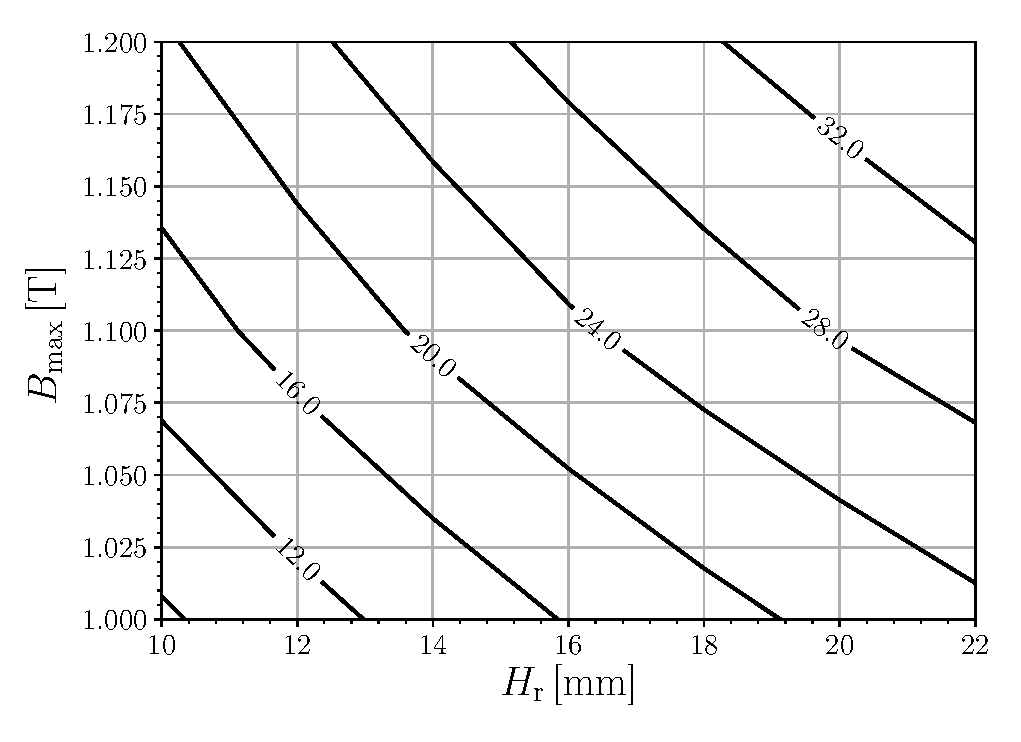
\includegraphics[width=5cm]{eta_H_regW30}\label{fig:eta_Hreg}}
  \caption{Performance of the AMR with varying regenerator height and high magnetic field, with fixed $F\ped{M} = F\ped{B} = \SI{70}{\percent}$ and $\Phi = 0.4$}
  \label{fig:qc-cop-eta-amr-height}
\end{figure}


\section{Final considerations}
\label{sec:final-considerations}

To the authors' knowledge, this is the first study where magnetic profiles for AMR model are mathematically modeled and the model parameters are changed in a systematic way.

The instantaneous profile yields higher cooling capacity, even by
reducing the blow fraction on rectified cosine, up to levels achieved by pumping and valving systems, mainly restricted by valve opening times

The ramp profile is a feasible approximation for the instantaneous
profile, and can be optimized for increasing cooling capacity.
In particular, by synchronizing the plateau durations between fluid
and magnetic profiles.

\begin{acknowledgements}
The authors duly acknowledge the financial support from CNPq (Grant no. 443696/2014-4), Capes (PTI program, Process no. 88887.194773/2018-00), Embraco and the EMBRAPII Unit Polo/UFSC.
\end{acknowledgements}

% BibTeX users please use one of
%\bibliographystyle{spbasic}      % basic style, author-year citations
%\bibliographystyle{spmpsci}      % mathematics and physical sciences
\bibliographystyle{spphys}       % APS-like style for physics

\bibliography{thermo-ref/Thermo-Foam-Ref,thermo-ref/thesis}

\end{document}

%%% Local Variables:
%%% mode: latex
%%% TeX-master: t
%%% End:
